% Options for packages loaded elsewhere
\PassOptionsToPackage{unicode}{hyperref}
\PassOptionsToPackage{hyphens}{url}
%
\documentclass[
]{article}
\usepackage{amsmath,amssymb}
\usepackage{lmodern}
\usepackage{iftex}
\ifPDFTeX
  \usepackage[T1]{fontenc}
  \usepackage[utf8]{inputenc}
  \usepackage{textcomp} % provide euro and other symbols
\else % if luatex or xetex
  \usepackage{unicode-math}
  \defaultfontfeatures{Scale=MatchLowercase}
  \defaultfontfeatures[\rmfamily]{Ligatures=TeX,Scale=1}
\fi
% Use upquote if available, for straight quotes in verbatim environments
\IfFileExists{upquote.sty}{\usepackage{upquote}}{}
\IfFileExists{microtype.sty}{% use microtype if available
  \usepackage[]{microtype}
  \UseMicrotypeSet[protrusion]{basicmath} % disable protrusion for tt fonts
}{}
\makeatletter
\@ifundefined{KOMAClassName}{% if non-KOMA class
  \IfFileExists{parskip.sty}{%
    \usepackage{parskip}
  }{% else
    \setlength{\parindent}{0pt}
    \setlength{\parskip}{6pt plus 2pt minus 1pt}}
}{% if KOMA class
  \KOMAoptions{parskip=half}}
\makeatother
\usepackage{xcolor}
\usepackage[margin=1in]{geometry}
\usepackage{color}
\usepackage{fancyvrb}
\newcommand{\VerbBar}{|}
\newcommand{\VERB}{\Verb[commandchars=\\\{\}]}
\DefineVerbatimEnvironment{Highlighting}{Verbatim}{commandchars=\\\{\}}
% Add ',fontsize=\small' for more characters per line
\usepackage{framed}
\definecolor{shadecolor}{RGB}{248,248,248}
\newenvironment{Shaded}{\begin{snugshade}}{\end{snugshade}}
\newcommand{\AlertTok}[1]{\textcolor[rgb]{0.94,0.16,0.16}{#1}}
\newcommand{\AnnotationTok}[1]{\textcolor[rgb]{0.56,0.35,0.01}{\textbf{\textit{#1}}}}
\newcommand{\AttributeTok}[1]{\textcolor[rgb]{0.77,0.63,0.00}{#1}}
\newcommand{\BaseNTok}[1]{\textcolor[rgb]{0.00,0.00,0.81}{#1}}
\newcommand{\BuiltInTok}[1]{#1}
\newcommand{\CharTok}[1]{\textcolor[rgb]{0.31,0.60,0.02}{#1}}
\newcommand{\CommentTok}[1]{\textcolor[rgb]{0.56,0.35,0.01}{\textit{#1}}}
\newcommand{\CommentVarTok}[1]{\textcolor[rgb]{0.56,0.35,0.01}{\textbf{\textit{#1}}}}
\newcommand{\ConstantTok}[1]{\textcolor[rgb]{0.00,0.00,0.00}{#1}}
\newcommand{\ControlFlowTok}[1]{\textcolor[rgb]{0.13,0.29,0.53}{\textbf{#1}}}
\newcommand{\DataTypeTok}[1]{\textcolor[rgb]{0.13,0.29,0.53}{#1}}
\newcommand{\DecValTok}[1]{\textcolor[rgb]{0.00,0.00,0.81}{#1}}
\newcommand{\DocumentationTok}[1]{\textcolor[rgb]{0.56,0.35,0.01}{\textbf{\textit{#1}}}}
\newcommand{\ErrorTok}[1]{\textcolor[rgb]{0.64,0.00,0.00}{\textbf{#1}}}
\newcommand{\ExtensionTok}[1]{#1}
\newcommand{\FloatTok}[1]{\textcolor[rgb]{0.00,0.00,0.81}{#1}}
\newcommand{\FunctionTok}[1]{\textcolor[rgb]{0.00,0.00,0.00}{#1}}
\newcommand{\ImportTok}[1]{#1}
\newcommand{\InformationTok}[1]{\textcolor[rgb]{0.56,0.35,0.01}{\textbf{\textit{#1}}}}
\newcommand{\KeywordTok}[1]{\textcolor[rgb]{0.13,0.29,0.53}{\textbf{#1}}}
\newcommand{\NormalTok}[1]{#1}
\newcommand{\OperatorTok}[1]{\textcolor[rgb]{0.81,0.36,0.00}{\textbf{#1}}}
\newcommand{\OtherTok}[1]{\textcolor[rgb]{0.56,0.35,0.01}{#1}}
\newcommand{\PreprocessorTok}[1]{\textcolor[rgb]{0.56,0.35,0.01}{\textit{#1}}}
\newcommand{\RegionMarkerTok}[1]{#1}
\newcommand{\SpecialCharTok}[1]{\textcolor[rgb]{0.00,0.00,0.00}{#1}}
\newcommand{\SpecialStringTok}[1]{\textcolor[rgb]{0.31,0.60,0.02}{#1}}
\newcommand{\StringTok}[1]{\textcolor[rgb]{0.31,0.60,0.02}{#1}}
\newcommand{\VariableTok}[1]{\textcolor[rgb]{0.00,0.00,0.00}{#1}}
\newcommand{\VerbatimStringTok}[1]{\textcolor[rgb]{0.31,0.60,0.02}{#1}}
\newcommand{\WarningTok}[1]{\textcolor[rgb]{0.56,0.35,0.01}{\textbf{\textit{#1}}}}
\usepackage{graphicx}
\makeatletter
\def\maxwidth{\ifdim\Gin@nat@width>\linewidth\linewidth\else\Gin@nat@width\fi}
\def\maxheight{\ifdim\Gin@nat@height>\textheight\textheight\else\Gin@nat@height\fi}
\makeatother
% Scale images if necessary, so that they will not overflow the page
% margins by default, and it is still possible to overwrite the defaults
% using explicit options in \includegraphics[width, height, ...]{}
\setkeys{Gin}{width=\maxwidth,height=\maxheight,keepaspectratio}
% Set default figure placement to htbp
\makeatletter
\def\fps@figure{htbp}
\makeatother
\setlength{\emergencystretch}{3em} % prevent overfull lines
\providecommand{\tightlist}{%
  \setlength{\itemsep}{0pt}\setlength{\parskip}{0pt}}
\setcounter{secnumdepth}{-\maxdimen} % remove section numbering
\ifLuaTeX
  \usepackage{selnolig}  % disable illegal ligatures
\fi
\IfFileExists{bookmark.sty}{\usepackage{bookmark}}{\usepackage{hyperref}}
\IfFileExists{xurl.sty}{\usepackage{xurl}}{} % add URL line breaks if available
\urlstyle{same} % disable monospaced font for URLs
\hypersetup{
  pdftitle={Trabajo Practico Regresión Avanzada},
  pdfauthor={Jose Valdes},
  hidelinks,
  pdfcreator={LaTeX via pandoc}}

\title{Trabajo Practico Regresión Avanzada}
\usepackage{etoolbox}
\makeatletter
\providecommand{\subtitle}[1]{% add subtitle to \maketitle
  \apptocmd{\@title}{\par {\large #1 \par}}{}{}
}
\makeatother
\subtitle{Regresión Lineal Simple}
\author{Jose Valdes}
\date{2023-06-05}

\begin{document}
\maketitle

{
\setcounter{tocdepth}{5}
\tableofcontents
}
\begin{Shaded}
\begin{Highlighting}[]
\CommentTok{\#limpio la memoria}
\FunctionTok{rm}\NormalTok{( }\AttributeTok{list=} \FunctionTok{ls}\NormalTok{(}\AttributeTok{all.names=} \ConstantTok{TRUE}\NormalTok{) )  }\CommentTok{\#remove all objects}
\FunctionTok{gc}\NormalTok{( }\AttributeTok{full=} \ConstantTok{TRUE}\NormalTok{ )                 }\CommentTok{\#garbage collection}
\end{Highlighting}
\end{Shaded}

\begin{verbatim}
##          used (Mb) gc trigger (Mb) max used (Mb)
## Ncells 465658 24.9    1008328 53.9   644245 34.5
## Vcells 844537  6.5    8388608 64.0  1635137 12.5
\end{verbatim}

Se realiza validación de la instalación de los paquetes necesarios para
ejecutar el script

\begin{Shaded}
\begin{Highlighting}[]
\CommentTok{\# Bibliotecas a cargar}

\NormalTok{check\_packages }\OtherTok{\textless{}{-}} \ControlFlowTok{function}\NormalTok{(packages) \{}
  \ControlFlowTok{if}\NormalTok{ (}\FunctionTok{all}\NormalTok{(packages }\SpecialCharTok{\%in\%} \FunctionTok{rownames}\NormalTok{(}\FunctionTok{installed.packages}\NormalTok{()))) \{}
    \ConstantTok{TRUE}
\NormalTok{  \} }\ControlFlowTok{else}\NormalTok{\{}
    \FunctionTok{cat}\NormalTok{(}
      \StringTok{"Instalar los siguientes packages antes de ejecutar el presente script}\SpecialCharTok{\textbackslash{}n}\StringTok{"}\NormalTok{,}
\NormalTok{      packages[}\SpecialCharTok{!}\NormalTok{(packages }\SpecialCharTok{\%in\%} \FunctionTok{rownames}\NormalTok{(}\FunctionTok{installed.packages}\NormalTok{()))],}
      \StringTok{"}\SpecialCharTok{\textbackslash{}n}\StringTok{"}
\NormalTok{    )}
\NormalTok{  \}}
\NormalTok{\}}
\NormalTok{packages\_needed }\OtherTok{\textless{}{-}} \FunctionTok{c}\NormalTok{(}\StringTok{"readxl"}\NormalTok{,}\StringTok{"ggplot2"}\NormalTok{,}\StringTok{"MVN"}\NormalTok{,}\StringTok{"gridExtra"}\NormalTok{,}\StringTok{"aod"}\NormalTok{,}\StringTok{"MASS"}\NormalTok{,}\StringTok{"carData"}\NormalTok{,}\StringTok{"car"}\NormalTok{)}

\CommentTok{\# Se llama a la funcion check\_packages}
\FunctionTok{check\_packages}\NormalTok{(packages\_needed)}
\end{Highlighting}
\end{Shaded}

\begin{verbatim}
## [1] TRUE
\end{verbatim}

\begin{Shaded}
\begin{Highlighting}[]
\FunctionTok{library}\NormalTok{(readxl)}
\FunctionTok{library}\NormalTok{(ggplot2)}
\FunctionTok{library}\NormalTok{(MVN)}
\FunctionTok{library}\NormalTok{(gridExtra)}
\FunctionTok{library}\NormalTok{(aod)}
\FunctionTok{library}\NormalTok{(MASS)}
\FunctionTok{library}\NormalTok{(carData)}
\FunctionTok{library}\NormalTok{(car)}
\end{Highlighting}
\end{Shaded}

\hypertarget{correlaciuxf3n}{%
\section{\texorpdfstring{{1.1.
Correlación}}{1.1. Correlación}}\label{correlaciuxf3n}}

\hypertarget{ejercicio-1.1.}{%
\subsection{Ejercicio 1.1.}\label{ejercicio-1.1.}}

En el archivo grasacerdos.xlsx se encuentran los datos del peso vivo
(PV, en Kg) y al espesor de grasa dorsal (EGD, en mm) de 30 lechones
elegidos al azar de una población de porcinos Duroc Jersey del Oeste de
la provincia de Buenos Aires. Se pide

\hypertarget{a}{%
\subsubsection{(a)}\label{a}}

Dibujar el diagrama de dispersión e interpretarlo.

\begin{Shaded}
\begin{Highlighting}[]
\FunctionTok{library}\NormalTok{(readxl)}
\FunctionTok{library}\NormalTok{(ggplot2)}
\FunctionTok{library}\NormalTok{(MVN)}
\FunctionTok{library}\NormalTok{(gridExtra)}

\NormalTok{grasacerdos}\OtherTok{\textless{}{-}}\FunctionTok{read\_excel}\NormalTok{(}\StringTok{"C:/Users/Josvaldes/Documents/Maestria/Austral/1ano/regresionAvanzada/TPRegresion/TPRegresion/grasacerdos.xlsx"}\NormalTok{)}
\FunctionTok{dim}\NormalTok{(grasacerdos)}
\end{Highlighting}
\end{Shaded}

\begin{verbatim}
## [1] 30  3
\end{verbatim}

\begin{Shaded}
\begin{Highlighting}[]
\FunctionTok{head}\NormalTok{(grasacerdos)}
\end{Highlighting}
\end{Shaded}

\begin{verbatim}
## # A tibble: 6 x 3
##     Obs PV    EGD  
##   <dbl> <chr> <chr>
## 1     1 56,81 16,19
## 2     2 70,40 22,00
## 3     3 71,73 19,52
## 4     4 75,10 31,00
## 5     5 79,65 23,58
## 6     6 51,43 16,58
\end{verbatim}

\begin{Shaded}
\begin{Highlighting}[]
\NormalTok{grasacerdos}\SpecialCharTok{$}\NormalTok{PV }\OtherTok{\textless{}{-}} \FunctionTok{as.numeric}\NormalTok{(}\FunctionTok{gsub}\NormalTok{(}\StringTok{","}\NormalTok{, }\StringTok{"."}\NormalTok{, grasacerdos}\SpecialCharTok{$}\NormalTok{PV))}
\NormalTok{grasacerdos}\SpecialCharTok{$}\NormalTok{EGD }\OtherTok{\textless{}{-}} \FunctionTok{as.numeric}\NormalTok{(}\FunctionTok{gsub}\NormalTok{(}\StringTok{","}\NormalTok{, }\StringTok{"."}\NormalTok{, grasacerdos}\SpecialCharTok{$}\NormalTok{EGD))}
\end{Highlighting}
\end{Shaded}

\begin{Shaded}
\begin{Highlighting}[]
\FunctionTok{ggplot}\NormalTok{(grasacerdos, }\FunctionTok{aes}\NormalTok{(PV, EGD)) }\SpecialCharTok{+}
  \FunctionTok{geom\_point}\NormalTok{() }\SpecialCharTok{+}
  \FunctionTok{theme\_minimal}\NormalTok{() }\SpecialCharTok{+}
  \FunctionTok{labs}\NormalTok{(}\AttributeTok{x =} \StringTok{"Peso de Cerdos"}\NormalTok{, }\AttributeTok{y =} \StringTok{"Grasa Dorsal"}\NormalTok{,}
       \AttributeTok{title =}\NormalTok{ (}\StringTok{"Diagrama de Dispersi\textbackslash{}u00F3n Peso de Cerdos vs Grasa Dorsal"}\NormalTok{)) }\CommentTok{\# se deja la letra "ó" con \textbackslash{}u00F3, que                                                                             es la representación Unicode de esa letra}
\end{Highlighting}
\end{Shaded}

\includegraphics{TP_files/figure-latex/unnamed-chunk-5-1.pdf}

No se observa corelación entre las variables

\hypertarget{b}{%
\subsubsection{(b)}\label{b}}

Calcular el coeficiente de correlación muestral y explíquelo.

\begin{Shaded}
\begin{Highlighting}[]
\NormalTok{biNormTest }\OtherTok{\textless{}{-}} \FunctionTok{mvn}\NormalTok{(grasacerdos, }\AttributeTok{mvnTest =} \StringTok{"hz"}\NormalTok{)}
\FunctionTok{print}\NormalTok{(biNormTest}\SpecialCharTok{$}\NormalTok{multivariateNormality)}
\end{Highlighting}
\end{Shaded}

\begin{verbatim}
##            Test        HZ   p value MVN
## 1 Henze-Zirkler 0.6379234 0.3891766 YES
\end{verbatim}

Por el resultado se puede sostener el supuesto de una distribución
normal bivariada para estas variables. En tal sentido, se procede a
realizar el test de Pearson para determinar la relación de las
variables:

\begin{Shaded}
\begin{Highlighting}[]
\NormalTok{corCoeff }\OtherTok{\textless{}{-}} \FunctionTok{cor}\NormalTok{(grasacerdos}\SpecialCharTok{$}\NormalTok{PV,grasacerdos}\SpecialCharTok{$}\NormalTok{EGD, }\AttributeTok{method =} \StringTok{"pearson"}\NormalTok{)}
\NormalTok{corCoeff}
\end{Highlighting}
\end{Shaded}

\begin{verbatim}
## [1] 0.2543434
\end{verbatim}

La prueba de correlación de Pearson muestra que existe una correlación
positiva débil entre las variables. Esto significa que hay una tendencia
a que los valores de las variables aumenten juntos, pero la relación no
es muy fuerte.

\hypertarget{c}{%
\subsubsection{(c)}\label{c}}

¿Hay suficiente evidencia para admitir asociación entre el peso y el
espesor de grasa? (α = 0,05). Verifique los supuestos para decidir el
indicador que va a utilizar.

Para determinar si hay suficiente evidencia para admitir una asociación
entre el peso y el espesor de grasa, es necesario verificar los
supuestos y luego utilizar un indicador apropiado para evaluar la
correlación entre las variables.

A continuación, se describen los supuestos que se deben verificar antes
de seleccionar el indicador:

1 - Supuesto de normalidad: Se debe verificar si las variables peso y
espesor de grasa siguen una distribución normal. Esto se puede hacer
mediante métodos gráficos, como histogramas o gráficos de Q-Q, y pruebas
estadísticas, como el test de normalidad (por ejemplo, el test de
Shapiro-Wilk).

\begin{Shaded}
\begin{Highlighting}[]
\FunctionTok{shapiro.test}\NormalTok{(grasacerdos}\SpecialCharTok{$}\NormalTok{PV)}
\end{Highlighting}
\end{Shaded}

\begin{verbatim}
## 
##  Shapiro-Wilk normality test
## 
## data:  grasacerdos$PV
## W = 0.97533, p-value = 0.6925
\end{verbatim}

\begin{Shaded}
\begin{Highlighting}[]
\FunctionTok{shapiro.test}\NormalTok{(grasacerdos}\SpecialCharTok{$}\NormalTok{EGD)}
\end{Highlighting}
\end{Shaded}

\begin{verbatim}
## 
##  Shapiro-Wilk normality test
## 
## data:  grasacerdos$EGD
## W = 0.98514, p-value = 0.9395
\end{verbatim}

\begin{Shaded}
\begin{Highlighting}[]
\FunctionTok{par}\NormalTok{(}\AttributeTok{mfrow =} \FunctionTok{c}\NormalTok{(}\DecValTok{1}\NormalTok{, }\DecValTok{2}\NormalTok{)) }
\FunctionTok{qqnorm}\NormalTok{(grasacerdos}\SpecialCharTok{$}\NormalTok{PV, }\AttributeTok{main =} \StringTok{"Peso"}\NormalTok{, }\AttributeTok{col =} \StringTok{"darkred"}\NormalTok{) }
\FunctionTok{qqline}\NormalTok{(grasacerdos}\SpecialCharTok{$}\NormalTok{PV) }
\FunctionTok{qqnorm}\NormalTok{(grasacerdos}\SpecialCharTok{$}\NormalTok{EGD, }\AttributeTok{main =} \StringTok{"Grasa dorsal"}\NormalTok{, }\AttributeTok{col =} \StringTok{"blue"}\NormalTok{) }
\FunctionTok{qqline}\NormalTok{(grasacerdos}\SpecialCharTok{$}\NormalTok{EGD)}
\end{Highlighting}
\end{Shaded}

\includegraphics{TP_files/figure-latex/unnamed-chunk-10-1.pdf}

\begin{Shaded}
\begin{Highlighting}[]
\FunctionTok{par}\NormalTok{(}\AttributeTok{mfrow =} \FunctionTok{c}\NormalTok{(}\DecValTok{1}\NormalTok{, }\DecValTok{2}\NormalTok{))}
\FunctionTok{hist}\NormalTok{(grasacerdos}\SpecialCharTok{$}\NormalTok{PV, }\AttributeTok{breaks =} \DecValTok{10}\NormalTok{, }\AttributeTok{main =} \StringTok{""}\NormalTok{, }\AttributeTok{xlab =} \StringTok{"Peso"}\NormalTok{, }\AttributeTok{border =} \StringTok{"darkred"}\NormalTok{) }
\FunctionTok{hist}\NormalTok{(grasacerdos}\SpecialCharTok{$}\NormalTok{EGD, }\AttributeTok{breaks =} \DecValTok{10}\NormalTok{, }\AttributeTok{main =} \StringTok{""}\NormalTok{, }\AttributeTok{xlab =} \StringTok{"Grasa dorsal"}\NormalTok{, }\AttributeTok{border =} \StringTok{"blue"}\NormalTok{)}
\end{Highlighting}
\end{Shaded}

\includegraphics{TP_files/figure-latex/unnamed-chunk-11-1.pdf}

\begin{Shaded}
\begin{Highlighting}[]
\FunctionTok{par}\NormalTok{(}\AttributeTok{bg=}\StringTok{"white"}\NormalTok{)}
\FunctionTok{pairs}\NormalTok{(grasacerdos) }\CommentTok{\# representa todos los diagramas de dispersión de a pares}
\end{Highlighting}
\end{Shaded}

\includegraphics{TP_files/figure-latex/unnamed-chunk-12-1.pdf}

2 - Supuesto de linealidad: Se debe verificar si la relación entre el
peso y el espesor de grasa es lineal. Esto se puede explorar mediante un
diagrama de dispersión o mediante técnicas de análisis exploratorio de
datos.

3 - Supuesto de homogeneidad de varianzas: Se debe verificar si la
varianza del espesor de grasa es constante en diferentes niveles de
peso. Esto se puede evaluar mediante gráficos de dispersión y pruebas
estadísticas, como el test de Levene.

Una vez que se han verificado los supuestos, puedes seleccionar un
indicador apropiado para evaluar la asociación entre el peso y el
espesor de grasa. Dado que estamos analizando una relación entre dos
variables continuas, el coeficiente de correlación de Pearson sería un
indicador adecuado.

Para determinar si hay suficiente evidencia para admitir la asociación
entre el peso y el espesor de grasa, se puede realizar una prueba de
hipótesis utilizando el coeficiente de correlación de Pearson. El
enunciado de las hipótesis sería:

Hipótesis nula (H0): No hay asociación entre el peso y el espesor de
grasa (ρ = 0). Hipótesis alternativa (HA): Hay asociación entre el peso
y el espesor de grasa (ρ ≠ 0).

\begin{Shaded}
\begin{Highlighting}[]
\NormalTok{corTest }\OtherTok{\textless{}{-}} \FunctionTok{cor.test}\NormalTok{(grasacerdos}\SpecialCharTok{$}\NormalTok{PV,grasacerdos}\SpecialCharTok{$}\NormalTok{EGD, }\AttributeTok{method =} \StringTok{"pearson"}\NormalTok{) }
\NormalTok{corTest}
\end{Highlighting}
\end{Shaded}

\begin{verbatim}
## 
##  Pearson's product-moment correlation
## 
## data:  grasacerdos$PV and grasacerdos$EGD
## t = 1.3916, df = 28, p-value = 0.175
## alternative hypothesis: true correlation is not equal to 0
## 95 percent confidence interval:
##  -0.1166112  0.5630217
## sample estimates:
##       cor 
## 0.2543434
\end{verbatim}

El resultado del test de correlación de Pearson como se mostró en el
punto b corresponde a una correlacion positiva baja entre las variables
y un P-valor de 0.1749942 que seria mayor que el nivel de significancia
\(\alpha\) = 0,05 de la prueba, por tal razon, no se puede afirmar la
presencia de una asociación significativa entre las variables.

\hypertarget{ejercicio-1.2.}{%
\subsection{Ejercicio 1.2.}\label{ejercicio-1.2.}}

Los datos del cuarteto de Anscombe se encuentran en el archivo
anscombe.xlsx

Se pide explorar los datos de la siguiente manera:

\hypertarget{a-1}{%
\subsubsection{(a)}\label{a-1}}

Graficar los cuatro pares de datos en un diagrama de dispersión cada
uno.

\begin{Shaded}
\begin{Highlighting}[]
\CommentTok{\# se observa que el archivo esta incompleto anscombe.xlsx (dimensiones 6x8), se busca en internet y se trabaja con Anscombe\textquotesingle{}s Quartet.xlsx (dimensiones 12x8)}
\NormalTok{anscombe}\OtherTok{\textless{}{-}}\FunctionTok{read\_excel}\NormalTok{(}\StringTok{"C:/Users/Josvaldes/Documents/Maestria/Austral/1ano/regresionAvanzada/TPRegresion/TPRegresion/Anscombe\textquotesingle{}s Quartet.xlsx"}\NormalTok{)}
\FunctionTok{dim}\NormalTok{(anscombe)}
\end{Highlighting}
\end{Shaded}

\begin{verbatim}
## [1] 11  8
\end{verbatim}

\begin{Shaded}
\begin{Highlighting}[]
\FunctionTok{head}\NormalTok{(anscombe)}
\end{Highlighting}
\end{Shaded}

\begin{verbatim}
## # A tibble: 6 x 8
##      X1    X2    X3    X4    X5    X6    X7    X8
##   <dbl> <dbl> <dbl> <dbl> <dbl> <dbl> <dbl> <dbl>
## 1    10  8.04    10  9.14    10  7.46     8  6.58
## 2     8  6.95     8  8.14     8  6.77     8  5.76
## 3    13  7.58    13  8.74    13 12.7      8  7.71
## 4     9  8.81     9  8.77     9  7.11     8  8.84
## 5    11  8.33    11  9.26    11  7.81     8  8.47
## 6    14  9.96    14  8.1     14  8.84     8  7.04
\end{verbatim}

\begin{Shaded}
\begin{Highlighting}[]
\NormalTok{dd1}\OtherTok{=}\FunctionTok{ggplot}\NormalTok{(anscombe, }\FunctionTok{aes}\NormalTok{(X1, X2)) }\SpecialCharTok{+} 
  \FunctionTok{geom\_point}\NormalTok{() }\SpecialCharTok{+} \FunctionTok{theme\_minimal}\NormalTok{() }\SpecialCharTok{+} \FunctionTok{labs}\NormalTok{(}\AttributeTok{title =} \StringTok{"Diagrama de Dispersi\textbackslash{}u00F3n X1 vs X2"}\NormalTok{)}
\NormalTok{dd1}
\end{Highlighting}
\end{Shaded}

\includegraphics{TP_files/figure-latex/unnamed-chunk-16-1.pdf}

\begin{Shaded}
\begin{Highlighting}[]
\NormalTok{dd2}\OtherTok{=}\FunctionTok{ggplot}\NormalTok{(anscombe, }\FunctionTok{aes}\NormalTok{(X3, X4)) }\SpecialCharTok{+} 
  \FunctionTok{geom\_point}\NormalTok{() }\SpecialCharTok{+} \FunctionTok{theme\_minimal}\NormalTok{() }\SpecialCharTok{+} \FunctionTok{labs}\NormalTok{(}\AttributeTok{title =} \StringTok{"Diagrama de Dispersi\textbackslash{}u00F3n X3 vs X4"}\NormalTok{)}
\NormalTok{dd2}
\end{Highlighting}
\end{Shaded}

\includegraphics{TP_files/figure-latex/unnamed-chunk-17-1.pdf}

\begin{Shaded}
\begin{Highlighting}[]
\NormalTok{dd3}\OtherTok{=}\FunctionTok{ggplot}\NormalTok{(anscombe, }\FunctionTok{aes}\NormalTok{(X5, X6)) }\SpecialCharTok{+} 
  \FunctionTok{geom\_point}\NormalTok{() }\SpecialCharTok{+} \FunctionTok{theme\_minimal}\NormalTok{() }\SpecialCharTok{+} \FunctionTok{labs}\NormalTok{(}\AttributeTok{title =} \StringTok{"Diagrama de Dispersi\textbackslash{}u00F3n X5 vs X6"}\NormalTok{)}
\NormalTok{dd3}
\end{Highlighting}
\end{Shaded}

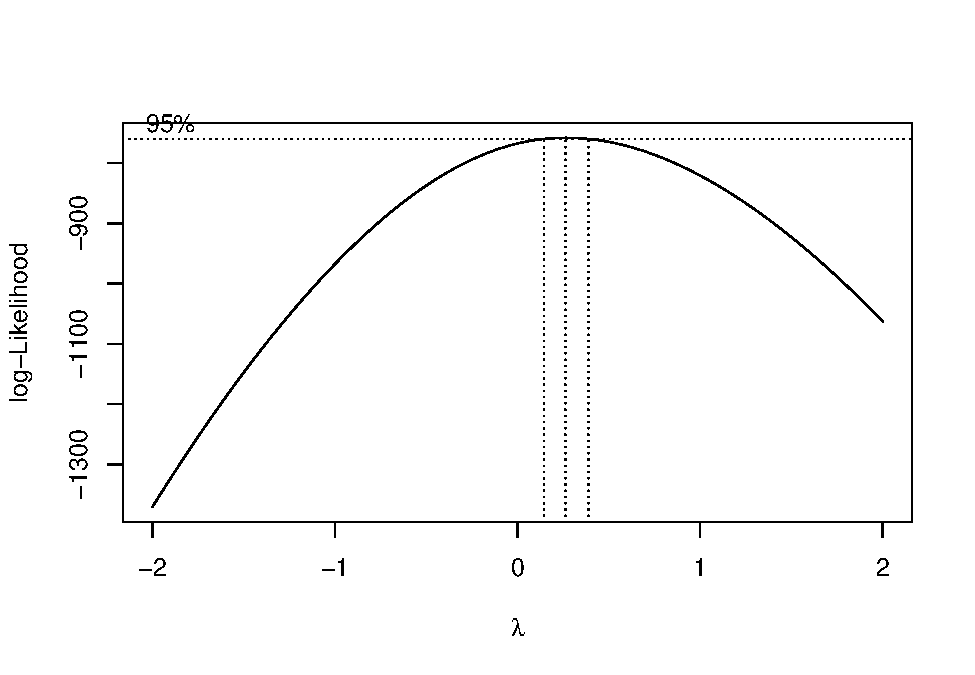
\includegraphics{TP_files/figure-latex/unnamed-chunk-18-1.pdf}

\begin{Shaded}
\begin{Highlighting}[]
\NormalTok{dd4}\OtherTok{=}\FunctionTok{ggplot}\NormalTok{(anscombe, }\FunctionTok{aes}\NormalTok{(X7, X8)) }\SpecialCharTok{+} 
  \FunctionTok{geom\_point}\NormalTok{() }\SpecialCharTok{+} \FunctionTok{theme\_minimal}\NormalTok{() }\SpecialCharTok{+} \FunctionTok{labs}\NormalTok{(}\AttributeTok{title =} \StringTok{"Diagrama de Dispersi\textbackslash{}u00F3n X7 vs X8"}\NormalTok{)}
\NormalTok{dd4}
\end{Highlighting}
\end{Shaded}

\includegraphics{TP_files/figure-latex/unnamed-chunk-19-1.pdf}

\begin{Shaded}
\begin{Highlighting}[]
\CommentTok{\#resumen}
\FunctionTok{grid.arrange}\NormalTok{(dd1,dd2,dd3,dd4, }\AttributeTok{ncol =} \DecValTok{2}\NormalTok{, }\AttributeTok{nrow =} \DecValTok{2}\NormalTok{)}
\end{Highlighting}
\end{Shaded}

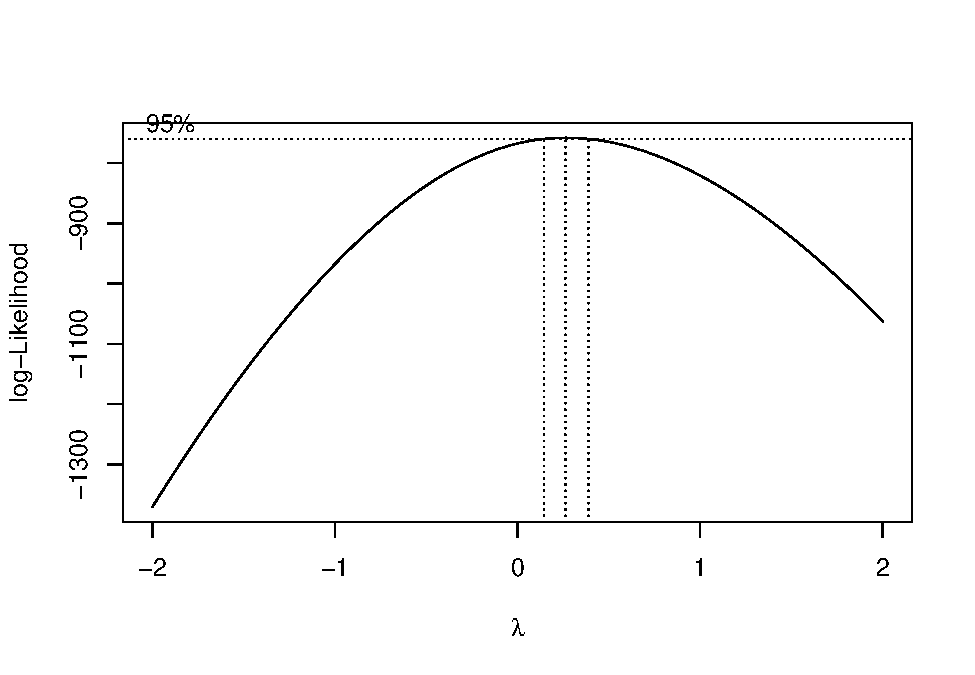
\includegraphics{TP_files/figure-latex/unnamed-chunk-20-1.pdf}

\hypertarget{b-1}{%
\subsubsection{(b)}\label{b-1}}

Hallar los valores medios de las variables para cada par de datos.

\begin{Shaded}
\begin{Highlighting}[]
\FunctionTok{colMeans}\NormalTok{(anscombe)}
\end{Highlighting}
\end{Shaded}

\begin{verbatim}
##       X1       X2       X3       X4       X5       X6       X7       X8 
## 9.000000 7.500909 9.000000 7.500909 9.000000 7.500000 9.000000 7.500909
\end{verbatim}

\hypertarget{c-1}{%
\subsubsection{(c)}\label{c-1}}

Hallar los valores de la dispersión para cada conjunto de datos.

\begin{Shaded}
\begin{Highlighting}[]
\FunctionTok{sapply}\NormalTok{(anscombe, sd)}
\end{Highlighting}
\end{Shaded}

\begin{verbatim}
##       X1       X2       X3       X4       X5       X6       X7       X8 
## 3.316625 2.031568 3.316625 2.031657 3.316625 2.030424 3.316625 2.030579
\end{verbatim}

\hypertarget{d}{%
\subsubsection{(d)}\label{d}}

Hallar el coeficiente muestral de correlación lineal en cada caso.

\begin{Shaded}
\begin{Highlighting}[]
\FunctionTok{mvn}\NormalTok{(}\AttributeTok{data =}\NormalTok{ anscombe[}\FunctionTok{c}\NormalTok{(}\DecValTok{1}\NormalTok{,}\DecValTok{2}\NormalTok{)], }\AttributeTok{mvnTest =} \StringTok{"hz"}\NormalTok{)}\SpecialCharTok{$}\NormalTok{multivariateNormality}\SpecialCharTok{$}\NormalTok{MVN}
\end{Highlighting}
\end{Shaded}

\begin{verbatim}
## [1] "YES"
\end{verbatim}

\begin{Shaded}
\begin{Highlighting}[]
\FunctionTok{mvn}\NormalTok{(}\AttributeTok{data =}\NormalTok{ anscombe[}\FunctionTok{c}\NormalTok{(}\DecValTok{3}\NormalTok{,}\DecValTok{4}\NormalTok{)], }\AttributeTok{mvnTest =} \StringTok{"hz"}\NormalTok{)}\SpecialCharTok{$}\NormalTok{multivariateNormality}\SpecialCharTok{$}\NormalTok{MVN}
\end{Highlighting}
\end{Shaded}

\begin{verbatim}
## [1] "NO"
\end{verbatim}

\begin{Shaded}
\begin{Highlighting}[]
\FunctionTok{mvn}\NormalTok{(}\AttributeTok{data =}\NormalTok{ anscombe[}\FunctionTok{c}\NormalTok{(}\DecValTok{5}\NormalTok{,}\DecValTok{6}\NormalTok{)], }\AttributeTok{mvnTest =} \StringTok{"hz"}\NormalTok{)}\SpecialCharTok{$}\NormalTok{multivariateNormality}\SpecialCharTok{$}\NormalTok{MVN}
\end{Highlighting}
\end{Shaded}

\begin{verbatim}
## [1] "NO"
\end{verbatim}

\begin{Shaded}
\begin{Highlighting}[]
\FunctionTok{mvn}\NormalTok{(}\AttributeTok{data =}\NormalTok{ anscombe[}\FunctionTok{c}\NormalTok{(}\DecValTok{7}\NormalTok{,}\DecValTok{8}\NormalTok{)], }\AttributeTok{mvnTest =} \StringTok{"hz"}\NormalTok{)}\SpecialCharTok{$}\NormalTok{multivariateNormality}\SpecialCharTok{$}\NormalTok{MVN}
\end{Highlighting}
\end{Shaded}

\begin{verbatim}
## [1] "NO"
\end{verbatim}

\begin{Shaded}
\begin{Highlighting}[]
\FunctionTok{cor.test}\NormalTok{(anscombe}\SpecialCharTok{$}\NormalTok{X1,anscombe}\SpecialCharTok{$}\NormalTok{X2,}\AttributeTok{method=}\StringTok{"pearson"}\NormalTok{)}\SpecialCharTok{$}\NormalTok{p.value}
\end{Highlighting}
\end{Shaded}

\begin{verbatim}
## [1] 0.002169629
\end{verbatim}

\begin{Shaded}
\begin{Highlighting}[]
\FunctionTok{cor.test}\NormalTok{(anscombe}\SpecialCharTok{$}\NormalTok{X3,anscombe}\SpecialCharTok{$}\NormalTok{X4,}\AttributeTok{method=}\StringTok{"spearman"}\NormalTok{)}\SpecialCharTok{$}\NormalTok{p.value}
\end{Highlighting}
\end{Shaded}

\begin{verbatim}
## [1] 0.02305887
\end{verbatim}

\begin{Shaded}
\begin{Highlighting}[]
\FunctionTok{cor.test}\NormalTok{(anscombe}\SpecialCharTok{$}\NormalTok{X5,anscombe}\SpecialCharTok{$}\NormalTok{X6,}\AttributeTok{method=}\StringTok{"spearman"}\NormalTok{)}\SpecialCharTok{$}\NormalTok{p.value}
\end{Highlighting}
\end{Shaded}

\begin{verbatim}
## [1] 0
\end{verbatim}

\begin{Shaded}
\begin{Highlighting}[]
\FunctionTok{cor.test}\NormalTok{(anscombe}\SpecialCharTok{$}\NormalTok{X7,anscombe}\SpecialCharTok{$}\NormalTok{X8,}\AttributeTok{method=}\StringTok{"spearman"}\NormalTok{)}\SpecialCharTok{$}\NormalTok{p.value}
\end{Highlighting}
\end{Shaded}

\begin{verbatim}
## Warning in cor.test.default(anscombe$X7, anscombe$X8, method = "spearman"):
## Cannot compute exact p-value with ties
\end{verbatim}

\begin{verbatim}
## [1] 0.1173068
\end{verbatim}

Debido al Warning obtenido (Cannot compute exact p-value with
ties{[}1{]} 0.1173068), se calcula el coeficiente de correlación con el
método de Spearman, aun así que el test de Henze-Zirkler dice como
resultado NO.

\begin{Shaded}
\begin{Highlighting}[]
\FunctionTok{cor.test}\NormalTok{(anscombe}\SpecialCharTok{$}\NormalTok{X7,anscombe}\SpecialCharTok{$}\NormalTok{X8,}\AttributeTok{method=}\StringTok{"pearson"}\NormalTok{)}\SpecialCharTok{$}\NormalTok{p.value}
\end{Highlighting}
\end{Shaded}

\begin{verbatim}
## [1] 0.002164602
\end{verbatim}

\hypertarget{e}{%
\subsubsection{(e)}\label{e}}

Observar, comentar y concluir.

Por los resultados obtenidos en el primer par de variables se utiliza el
coeficiente de correlación de Pearson y para los tres paredes restantes
el de Spearman. Aunque para la relación de variables X7 y X8 aunque se
obtuvo con test de Henze-Zirkler como resultado NO, se recibe una
warning por el cual se hace la prueba con el test de Pearson.

\hypertarget{modelo-lineal-simple}{%
\section{\texorpdfstring{{1.2. Modelo Lineal
Simple}}{1.2. Modelo Lineal Simple}}\label{modelo-lineal-simple}}

\hypertarget{ejercicio-1.3.}{%
\subsection{Ejercicio 1.3.}\label{ejercicio-1.3.}}

El archivo peso\_edad\_colest.xlsx disponible contiene registros
correspondientes a 25 individuos respecto de su peso, su edad y el nivel
de colesterol total en sangre.

Se pide:

\hypertarget{a-2}{%
\subsubsection{(a)}\label{a-2}}

Realizar el diagrama de dispersión de colesterol en función de la edad y
de colesterol en función de peso. Le parece adecuado ajustar un modelo
lineal para alguno de estos dos pares de variables?

\begin{Shaded}
\begin{Highlighting}[]
\CommentTok{\#Se cargan los datos}
\NormalTok{colesterol }\OtherTok{\textless{}{-}} \FunctionTok{read\_excel}\NormalTok{(}\StringTok{\textquotesingle{}peso\_edad\_colest.xlsx\textquotesingle{}}\NormalTok{)}

\CommentTok{\#Se visualizan la estructura}
\FunctionTok{head}\NormalTok{(colesterol)}
\end{Highlighting}
\end{Shaded}

\begin{verbatim}
## # A tibble: 6 x 3
##    peso  edad colest
##   <dbl> <dbl>  <dbl>
## 1    84    46    354
## 2    73    20    190
## 3    65    52    405
## 4    70    30    263
## 5    76    57    451
## 6    69    25    302
\end{verbatim}

Se realizan los diagramas de dispersión solicitados

\begin{Shaded}
\begin{Highlighting}[]
\CommentTok{\#Diagrama de dispersión colesterol en función de la edad}
\NormalTok{dd112}\OtherTok{=}\FunctionTok{ggplot}\NormalTok{(colesterol, }\FunctionTok{aes}\NormalTok{(edad, colest)) }\SpecialCharTok{+} 
  \FunctionTok{geom\_point}\NormalTok{() }\SpecialCharTok{+} \FunctionTok{theme\_minimal}\NormalTok{() }\SpecialCharTok{+} \FunctionTok{labs}\NormalTok{(}\AttributeTok{title =} \StringTok{"Diagrama de Dispersi\textbackslash{}u00F3n edad vs colesterol"}\NormalTok{)}
\NormalTok{dd112}
\end{Highlighting}
\end{Shaded}

\includegraphics{TP_files/figure-latex/unnamed-chunk-26-1.pdf}

\begin{Shaded}
\begin{Highlighting}[]
\CommentTok{\#Diagrama de dispersión colesterol en función del peso}
\NormalTok{dd212}\OtherTok{=}\FunctionTok{ggplot}\NormalTok{(colesterol, }\FunctionTok{aes}\NormalTok{(peso, colest)) }\SpecialCharTok{+} 
  \FunctionTok{geom\_point}\NormalTok{() }\SpecialCharTok{+} \FunctionTok{theme\_minimal}\NormalTok{() }\SpecialCharTok{+} \FunctionTok{labs}\NormalTok{(}\AttributeTok{title =} \StringTok{"Diagrama de Dispersi\textbackslash{}u00F3n peso vs colesterol"}\NormalTok{)}
\NormalTok{dd212}
\end{Highlighting}
\end{Shaded}

\includegraphics{TP_files/figure-latex/unnamed-chunk-27-1.pdf}

Por las gráficas se podría pensar que se ajuste un modelo lineal entre
las variables edad y colesterol.

\hypertarget{b-2}{%
\subsubsection{(b)}\label{b-2}}

Estime los coeficientes del modelo lineal para el colesterol en función
de la edad.

Coeficientes

\begin{Shaded}
\begin{Highlighting}[]
\CommentTok{\#Modelo lineal para el colesterol en función de la edad.}
\NormalTok{model }\OtherTok{\textless{}{-}} \FunctionTok{lm}\NormalTok{(colest }\SpecialCharTok{\textasciitilde{}}\NormalTok{ edad, }\AttributeTok{data =}\NormalTok{ colesterol)}
\NormalTok{model}\SpecialCharTok{$}\NormalTok{coefficients}
\end{Highlighting}
\end{Shaded}

\begin{verbatim}
## (Intercept)        edad 
##   95.502004    5.670842
\end{verbatim}

Grafica del modelo y las bandas de error estándar alrededor de la línea
de regresión

\begin{Shaded}
\begin{Highlighting}[]
\NormalTok{(dd112}\SpecialCharTok{+} \FunctionTok{geom\_smooth}\NormalTok{(}\AttributeTok{method =} \StringTok{"lm"}\NormalTok{, }\AttributeTok{se =} \ConstantTok{TRUE}\NormalTok{, }\AttributeTok{color =} \StringTok{"black"}\NormalTok{) )}
\end{Highlighting}
\end{Shaded}

\begin{verbatim}
## `geom_smooth()` using formula = 'y ~ x'
\end{verbatim}

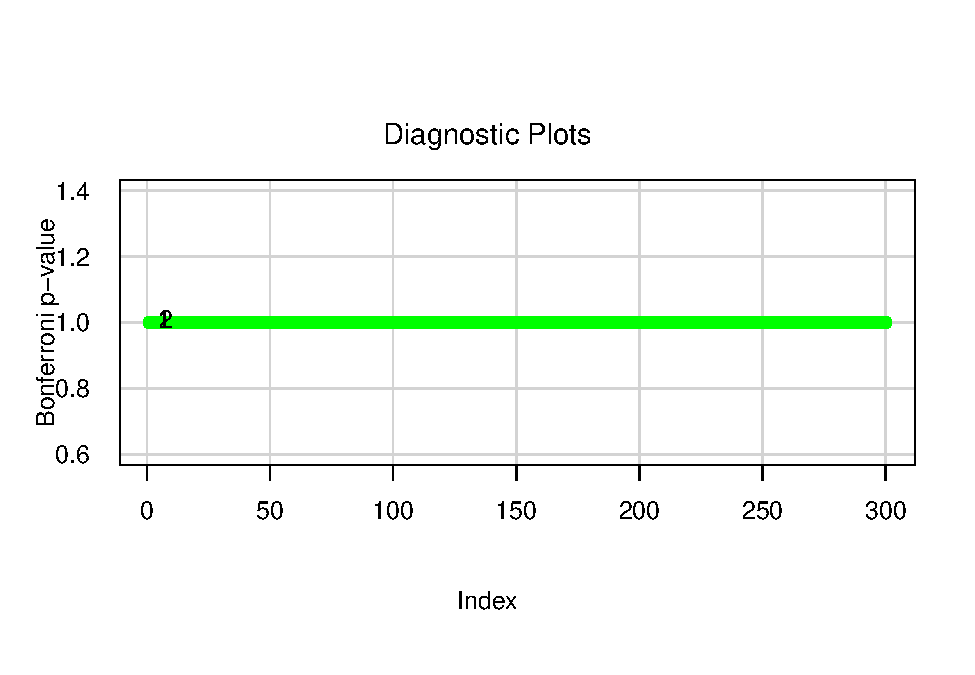
\includegraphics{TP_files/figure-latex/unnamed-chunk-29-1.pdf}

\hypertarget{c-2}{%
\subsubsection{(c)}\label{c-2}}

Estime intervalos de confianza del 95\% para los coeficientes del modelo
y compare estos resultados con el test de Wald para los coeficientes. Le
parece que hay asociación entre estos test y el test de la regresión?

\begin{Shaded}
\begin{Highlighting}[]
\NormalTok{ic }\OtherTok{\textless{}{-}} \FunctionTok{confint}\NormalTok{(model, }\AttributeTok{level =} \FloatTok{0.95}\NormalTok{)}
\NormalTok{ic}
\end{Highlighting}
\end{Shaded}

\begin{verbatim}
##                 2.5 %     97.5 %
## (Intercept) 41.190390 149.813618
## edad         4.358216   6.983467
\end{verbatim}

Test de Wald

\begin{Shaded}
\begin{Highlighting}[]
\FunctionTok{library}\NormalTok{(aod)}
\FunctionTok{coef}\NormalTok{(model)}
\end{Highlighting}
\end{Shaded}

\begin{verbatim}
## (Intercept)        edad 
##   95.502004    5.670842
\end{verbatim}

\begin{Shaded}
\begin{Highlighting}[]
\NormalTok{testWald}\OtherTok{=}\FunctionTok{wald.test}\NormalTok{(}\AttributeTok{Sigma =} \FunctionTok{vcov}\NormalTok{(model), }\AttributeTok{b =} \FunctionTok{coef}\NormalTok{(model), }\AttributeTok{Terms =} \DecValTok{1}\NormalTok{)}
\NormalTok{testWald}
\end{Highlighting}
\end{Shaded}

\begin{verbatim}
## Wald test:
## ----------
## 
## Chi-squared test:
## X2 = 13.2, df = 1, P(> X2) = 0.00028
\end{verbatim}

Las anteriores salidas muestra los coeficientes estimados del modelo de
regresión lineal y los resultados del test de Wald para evaluar la
significancia de los coeficientes.

Los coeficientes del modelo indican lo siguiente:

\begin{itemize}
\tightlist
\item
  El coeficiente de intercepto (Intercept) es de aproximadamente
  95.502004.
\item
  El coeficiente para la variable ``edad'' es de aproximadamente
  5.670842.
\end{itemize}

El test de Wald se utiliza para evaluar la significancia estadística de
los coeficientes del modelo. En este caso, se realiza el test de Wald
para el coeficiente del intercepto (intercept). El resultado del test
muestra que el estadístico de prueba chi-cuadrado (X2) es de 13.2, con 1
grado de libertad y un valor p (P(\textgreater X2)) de 0.00028.

Se puede concluir lo siguiente:

El coeficiente de intercepto es significativamente diferente de cero,
debido a que el valor p es muy pequeño (0.00028). Esto indica que hay
evidencia de una asociación entre la variable de respuesta y la variable
de intercepto.

En cuanto al coeficiente de la variable ``edad'', se realizan los
siguientes cancululos para obtener el test de wald:

\begin{Shaded}
\begin{Highlighting}[]
\CommentTok{\# Se obtiene la matriz de varianza{-}covarianza de los coeficientes del modelo}
\NormalTok{vcov\_model }\OtherTok{\textless{}{-}} \FunctionTok{vcov}\NormalTok{(model)}

\CommentTok{\# Se obtienen los coeficientes estimados del modelo}
\NormalTok{coef\_model }\OtherTok{\textless{}{-}} \FunctionTok{coef}\NormalTok{(model)}

\CommentTok{\# Calculo del estadístico de prueba utilizando la fórmula del test de Wald:}
\NormalTok{wald\_stat }\OtherTok{\textless{}{-}}\NormalTok{ (coef\_model[}\StringTok{"edad"}\NormalTok{] }\SpecialCharTok{{-}} \DecValTok{0}\NormalTok{) }\SpecialCharTok{/} \FunctionTok{sqrt}\NormalTok{(vcov\_model[}\StringTok{"edad"}\NormalTok{, }\StringTok{"edad"}\NormalTok{])}

\CommentTok{\# Calculo del valor p correspondiente al estadístico de prueba}
\NormalTok{p\_value }\OtherTok{\textless{}{-}} \DecValTok{1} \SpecialCharTok{{-}} \FunctionTok{pchisq}\NormalTok{(wald\_stat}\SpecialCharTok{\^{}}\DecValTok{2}\NormalTok{, }\AttributeTok{df =} \DecValTok{1}\NormalTok{)}

\CommentTok{\# Imprimir resultado}
\FunctionTok{cat}\NormalTok{(}\StringTok{"Test de Wald para la variable \textquotesingle{}edad\textquotesingle{}:}\SpecialCharTok{\textbackslash{}n}\StringTok{"}\NormalTok{)}
\end{Highlighting}
\end{Shaded}

\begin{verbatim}
## Test de Wald para la variable 'edad':
\end{verbatim}

\begin{Shaded}
\begin{Highlighting}[]
\FunctionTok{cat}\NormalTok{(}\StringTok{"{-}{-}{-}{-}{-}{-}{-}{-}{-}{-}{-}{-}{-}{-}{-}{-}{-}{-}{-}{-}{-}{-}{-}{-}}\SpecialCharTok{\textbackslash{}n}\StringTok{"}\NormalTok{)}
\end{Highlighting}
\end{Shaded}

\begin{verbatim}
## ------------------------
\end{verbatim}

\begin{Shaded}
\begin{Highlighting}[]
\FunctionTok{cat}\NormalTok{(}\StringTok{"Estadístico de prueba:"}\NormalTok{, wald\_stat, }\StringTok{"}\SpecialCharTok{\textbackslash{}n}\StringTok{"}\NormalTok{)}
\end{Highlighting}
\end{Shaded}

\begin{verbatim}
## Estadístico de prueba: 8.937073
\end{verbatim}

\begin{Shaded}
\begin{Highlighting}[]
\FunctionTok{cat}\NormalTok{(}\StringTok{"Valor p:"}\NormalTok{, p\_value, }\StringTok{"}\SpecialCharTok{\textbackslash{}n}\StringTok{"}\NormalTok{)}
\end{Highlighting}
\end{Shaded}

\begin{verbatim}
## Valor p: 0
\end{verbatim}

En resumen, hay evidencia de asociación entre el coeficiente de
intercepto y la variable de respuesta según el test de Wald.Para la
variable ``edad'' se tiene un estadístico de prueba de 8.937073 y un
valor p de 0. Esto indica que hay evidencia significativa para rechazar
la hipótesis nula de que el coeficiente de ``edad'' sea igual a cero.

\hypertarget{d-1}{%
\subsubsection{(d)}\label{d-1}}

A partir de esta recta estime los valores de E(Y ) para x = 25 años y x
= 48 años. Podría estimarse el valor de E(Y ) para x = 80 años?

Para estimar los valores de E(Y) para diferentes valores de x utilizando
la recta ajustada en el modelo de regresión, se pueden utilizar los
coeficientes del modelo.

En este caso, los coeficientes del modelo son:

Intercepto: 95.502004 Coeficiente para la variable ``edad'': 5.670842

E(Y) = Intercepto + Coeficiente * x

\begin{Shaded}
\begin{Highlighting}[]
\FunctionTok{predict}\NormalTok{(model, }\AttributeTok{newdata =} \FunctionTok{data.frame}\NormalTok{(}\AttributeTok{edad =} \FunctionTok{c}\NormalTok{(}\DecValTok{25}\NormalTok{,}\DecValTok{80}\NormalTok{)))}
\end{Highlighting}
\end{Shaded}

\begin{verbatim}
##        1        2 
## 237.2730 549.1693
\end{verbatim}

{Sin embargo, para valores de x más allá del rango de los datos
observados, como x = 80 años, la extrapolación puede no ser confiable.
La recta ajustada se basa en los datos observados y su validez puede
estar limitada a ese rango. Por lo tanto, no se recomienda estimar el
valor de E(Y) para x = 80 años utilizando este modelo de regresión.}

\hypertarget{e-1}{%
\subsubsection{(e)}\label{e-1}}

Testee la normalidad de los residuos y haga un gráfico para ver si son
homocedásticos.

\begin{Shaded}
\begin{Highlighting}[]
\CommentTok{\# Prueba de normalidad de Shapiro{-}Wilk }
\NormalTok{residuos }\OtherTok{\textless{}{-}} \FunctionTok{residuals}\NormalTok{(model)}
\FunctionTok{shapiro.test}\NormalTok{(residuos)}
\end{Highlighting}
\end{Shaded}

\begin{verbatim}
## 
##  Shapiro-Wilk normality test
## 
## data:  residuos
## W = 0.96478, p-value = 0.5175
\end{verbatim}

{El resultado de esta prueba proporciona un valor p que indica que no
hay suficiente evidencia para rechazar la hipótesis nula de normalidad
de los residuos. Como el valor p es mayor que un umbral de significancia
(por ejemplo, 0.05), se puede concluir que los residuos siguen una
distribución normal.}

Grafico de los residuos del modelo

\begin{Shaded}
\begin{Highlighting}[]
\FunctionTok{plot}\NormalTok{(residuos }\SpecialCharTok{\textasciitilde{}} \FunctionTok{fitted.values}\NormalTok{(model), }\AttributeTok{ylab =} \StringTok{"Residuos"}\NormalTok{, }\AttributeTok{xlab =} \StringTok{"Valores ajustados"}\NormalTok{)}
\FunctionTok{abline}\NormalTok{(}\AttributeTok{h =} \DecValTok{0}\NormalTok{, }\AttributeTok{col =} \StringTok{"red"}\NormalTok{)}
\end{Highlighting}
\end{Shaded}

\includegraphics{TP_files/figure-latex/unnamed-chunk-35-1.pdf}

Grafico con lineas:

\begin{Shaded}
\begin{Highlighting}[]
\NormalTok{colest2}\OtherTok{\textless{}{-}}\NormalTok{colesterol}
\NormalTok{colest2}\SpecialCharTok{$}\NormalTok{prediccion }\OtherTok{\textless{}{-}}\NormalTok{ model}\SpecialCharTok{$}\NormalTok{fitted.values }
\NormalTok{colest2}\SpecialCharTok{$}\NormalTok{residuos }\OtherTok{\textless{}{-}}\NormalTok{ model}\SpecialCharTok{$}\NormalTok{residuals}

\FunctionTok{ggplot}\NormalTok{(}\AttributeTok{data =}\NormalTok{ colest2, }\FunctionTok{aes}\NormalTok{(}\AttributeTok{x =}\NormalTok{ prediccion, }\AttributeTok{y =}\NormalTok{ residuos)) }\SpecialCharTok{+} 
  \FunctionTok{geom\_point}\NormalTok{(}\FunctionTok{aes}\NormalTok{(}\AttributeTok{color =}\NormalTok{ residuos)) }\SpecialCharTok{+} 
  \FunctionTok{scale\_color\_gradient2}\NormalTok{(}\AttributeTok{low =} \StringTok{"blue3"}\NormalTok{, }\AttributeTok{mid =} \StringTok{"grey"}\NormalTok{, }\AttributeTok{high =} \StringTok{"red"}\NormalTok{) }\SpecialCharTok{+} 
  \FunctionTok{geom\_hline}\NormalTok{(}\AttributeTok{yintercept =} \DecValTok{0}\NormalTok{) }\SpecialCharTok{+} \FunctionTok{geom\_segment}\NormalTok{(}\FunctionTok{aes}\NormalTok{(}\AttributeTok{xend =}\NormalTok{ prediccion, }\AttributeTok{yend =} \DecValTok{0}\NormalTok{), }\AttributeTok{alpha =} \FloatTok{0.2}\NormalTok{) }\SpecialCharTok{+} 
  \FunctionTok{labs}\NormalTok{(}\AttributeTok{title =} \StringTok{"Distribución de los residuos"}\NormalTok{, }\AttributeTok{x =} \StringTok{"predicción modelo"}\NormalTok{, }\AttributeTok{y =} \StringTok{"residuo"}\NormalTok{) }\SpecialCharTok{+} 
  \FunctionTok{theme\_bw}\NormalTok{() }\SpecialCharTok{+} 
  \FunctionTok{theme}\NormalTok{(}\AttributeTok{plot.title =} \FunctionTok{element\_text}\NormalTok{(}\AttributeTok{hjust =} \FloatTok{0.5}\NormalTok{), }\AttributeTok{legend.position =} \StringTok{"none"}\NormalTok{)}
\end{Highlighting}
\end{Shaded}

\includegraphics{TP_files/figure-latex/unnamed-chunk-36-1.pdf}

Grafico con histograma:

\begin{Shaded}
\begin{Highlighting}[]
\FunctionTok{ggplot}\NormalTok{(}\AttributeTok{data =}\NormalTok{ colest2, }\FunctionTok{aes}\NormalTok{(}\AttributeTok{x =}\NormalTok{ residuos)) }\SpecialCharTok{+} \FunctionTok{geom\_histogram}\NormalTok{(}\FunctionTok{aes}\NormalTok{(}\AttributeTok{y =} \FunctionTok{after\_stat}\NormalTok{(density))) }\SpecialCharTok{+} 
  \FunctionTok{labs}\NormalTok{(}\AttributeTok{title =} \StringTok{"Histograma de los residuos"}\NormalTok{) }\SpecialCharTok{+} \FunctionTok{theme\_bw}\NormalTok{() }\SpecialCharTok{+} 
  \FunctionTok{theme}\NormalTok{(}\AttributeTok{plot.title =} \FunctionTok{element\_text}\NormalTok{(}\AttributeTok{hjust =} \FloatTok{0.5}\NormalTok{))}
\end{Highlighting}
\end{Shaded}

\begin{verbatim}
## `stat_bin()` using `bins = 30`. Pick better value with `binwidth`.
\end{verbatim}

\includegraphics{TP_files/figure-latex/unnamed-chunk-37-1.pdf}

Grafico QQ

\begin{Shaded}
\begin{Highlighting}[]
\FunctionTok{qqnorm}\NormalTok{(model}\SpecialCharTok{$}\NormalTok{residuals, }\AttributeTok{main =} \StringTok{"Residuos del modelo"}\NormalTok{, }\AttributeTok{col =} \StringTok{"darkred"}\NormalTok{) }
\FunctionTok{qqline}\NormalTok{(model}\SpecialCharTok{$}\NormalTok{residuals) }
\end{Highlighting}
\end{Shaded}

\includegraphics{TP_files/figure-latex/unnamed-chunk-38-1.pdf}

{ De los resultados anteriores se puede suponer que los residuos del
modelo siguen una distribución normal y no son homocedasticos.}

\hypertarget{transformaciuxf3n-de-variables}{%
\section{\texorpdfstring{{ 1.3. Transformación de
Variables}}{ 1.3. Transformación de Variables}}\label{transformaciuxf3n-de-variables}}

\hypertarget{ejercicio-1.4.}{%
\subsection{Ejercicio 1.4.}\label{ejercicio-1.4.}}

{ Una empresa desarrolló un sistema de energía solar para calentar el
agua para una caldera que es parte del sistema de energía del proceso
productivo. Existe el interés de controlar la estabilidad del sistema,
para ello se monitorea el mismo y se registran los datos cada hora. Los
datos se encuentran disponibles en el archivo energia.xlsx}

\hypertarget{a-3}{%
\subsubsection{(a)}\label{a-3}}

Realizar el diagrama de dispersión y evaluar si un modelo de regresión
lineal es adecuado.

\begin{Shaded}
\begin{Highlighting}[]
\CommentTok{\# Se cargan los datos}
\NormalTok{energia }\OtherTok{\textless{}{-}} \FunctionTok{read\_excel}\NormalTok{(}\StringTok{\textquotesingle{}energia.xlsx\textquotesingle{}}\NormalTok{)}

\CommentTok{\#Se visualizan la estructura}
\FunctionTok{head}\NormalTok{(energia)}
\end{Highlighting}
\end{Shaded}

\begin{verbatim}
## # A tibble: 6 x 2
##    Hora Energía
##   <dbl>   <dbl>
## 1     1     598
## 2     2     527
## 3     3     530
## 4     4     528
## 5     5     452
## 6     6     497
\end{verbatim}

\begin{Shaded}
\begin{Highlighting}[]
\CommentTok{\#Dimensiones}
\FunctionTok{dim}\NormalTok{(energia)}
\end{Highlighting}
\end{Shaded}

\begin{verbatim}
## [1] 48  2
\end{verbatim}

Diagrama de dispersión

\begin{Shaded}
\begin{Highlighting}[]
\CommentTok{\#Diagrama de dispersión colesterol en función del peso}
\NormalTok{dd14}\OtherTok{=}\FunctionTok{ggplot}\NormalTok{(energia, }\FunctionTok{aes}\NormalTok{(Hora, Energía)) }\SpecialCharTok{+} 
  \FunctionTok{geom\_point}\NormalTok{() }\SpecialCharTok{+} \FunctionTok{theme\_minimal}\NormalTok{() }\SpecialCharTok{+} \FunctionTok{labs}\NormalTok{(}\AttributeTok{title =} \StringTok{"Diagrama de dispersi\textbackslash{}u00F3n Hora vs Energía"}\NormalTok{)}
\NormalTok{dd14}
\end{Highlighting}
\end{Shaded}

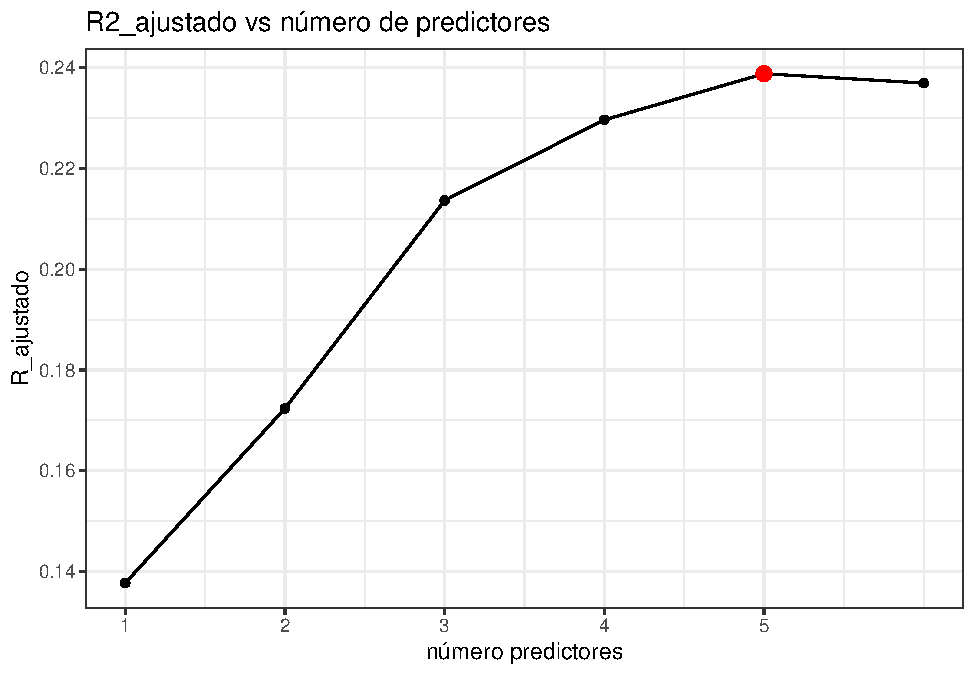
\includegraphics{TP_files/figure-latex/unnamed-chunk-41-1.pdf}

\begin{Shaded}
\begin{Highlighting}[]
\CommentTok{\# Validación de una distribución normal bivariada para estas variables}
\NormalTok{biNormTest14 }\OtherTok{\textless{}{-}} \FunctionTok{mvn}\NormalTok{(energia, }\AttributeTok{mvnTest =} \StringTok{"hz"}\NormalTok{)}
\NormalTok{biNormTest14 }
\end{Highlighting}
\end{Shaded}

\begin{verbatim}
## $multivariateNormality
##            Test       HZ     p value MVN
## 1 Henze-Zirkler 1.355059 0.002347283  NO
## 
## $univariateNormality
##               Test  Variable Statistic   p value Normality
## 1 Anderson-Darling   Hora       0.5128    0.1849    YES   
## 2 Anderson-Darling  Energía     1.1299    0.0053    NO    
## 
## $Descriptives
##          n   Mean  Std.Dev Median Min Max   25th   75th     Skew   Kurtosis
## Hora    48  24.50 14.00000   24.5   1  48  12.75  36.25 0.000000 -1.2752179
## Energía 48 504.25 93.07615  482.5 375 782 444.50 535.50 1.032494  0.8324672
\end{verbatim}

Por arrojar un resultado de MVN NO se realiza el test de Spearman

\begin{Shaded}
\begin{Highlighting}[]
\FunctionTok{cor.test}\NormalTok{(energia}\SpecialCharTok{$}\NormalTok{Hora,energia}\SpecialCharTok{$}\NormalTok{Energía,}\AttributeTok{method=}\StringTok{"spearman"}\NormalTok{)}\SpecialCharTok{$}\NormalTok{p.value}
\end{Highlighting}
\end{Shaded}

\begin{verbatim}
## Warning in cor.test.default(energia$Hora, energia$Energía, method =
## "spearman"): Cannot compute exact p-value with ties
\end{verbatim}

\begin{verbatim}
## [1] 0.806419
\end{verbatim}

\begin{Shaded}
\begin{Highlighting}[]
\CommentTok{\# métodos robustos para manejar empates}
\FunctionTok{cor.test}\NormalTok{(energia}\SpecialCharTok{$}\NormalTok{Hora, energia}\SpecialCharTok{$}\NormalTok{Energía, }\AttributeTok{method =} \StringTok{"spearman"}\NormalTok{, }\AttributeTok{exact =} \ConstantTok{FALSE}\NormalTok{)}
\end{Highlighting}
\end{Shaded}

\begin{verbatim}
## 
##  Spearman's rank correlation rho
## 
## data:  energia$Hora and energia$Energía
## S = 19093, p-value = 0.8064
## alternative hypothesis: true rho is not equal to 0
## sample estimates:
##         rho 
## -0.03631528
\end{verbatim}

La salida corresponde a la prueba de correlación de rangos de Spearman y
se puede interpretar de la siguiente manera:

\begin{itemize}
\item
  La primera línea indica que se realizó la prueba de correlación de
  rangos de Spearman en los datos de las variables ``Hora'' y
  ``Energía'' del dataframe ``energia''.
\item
  El valor de S es 19093, que es la suma de los cuadrados de las
  diferencias entre los rangos de las dos variables.
\item
  El valor p es 0.8064, que es el valor p obtenido de la prueba de
  hipótesis. En este caso, como el valor p es mayor que 0.05 (nivel de
  significancia comúnmente utilizado), no hay suficiente evidencia para
  rechazar la hipótesis nula de que no hay correlación entre las dos
  variables.
\item
  La hipótesis alternativa indica que el verdadero coeficiente de
  correlación rho no es igual a cero.
\item
  La estimación de rho basada en la muestra es -0.03631528, lo que
  indica una correlación negativa muy débil entre las dos variables.
\end{itemize}

En resumen, la salida sugiere que no hay evidencia suficiente para
concluir que hay una correlación significativa entre las variables
``Hora'' y ``Energía'' en el conjunto de datos analizado.

\hypertarget{b-3}{%
\subsubsection{(b)}\label{b-3}}

Estimar un modelo lineal y verificar la normalidad de los residuos del
mismo.

\begin{Shaded}
\begin{Highlighting}[]
\NormalTok{model14 }\OtherTok{=} \FunctionTok{lm}\NormalTok{(Energía }\SpecialCharTok{\textasciitilde{}}\NormalTok{ Hora, }\AttributeTok{data=}\NormalTok{energia)}
\FunctionTok{summary}\NormalTok{(model14)}
\end{Highlighting}
\end{Shaded}

\begin{verbatim}
## 
## Call:
## lm(formula = Energía ~ Hora, data = energia)
## 
## Residuals:
##     Min      1Q  Median      3Q     Max 
## -131.12  -60.60  -24.31   37.29  273.84 
## 
## Coefficients:
##             Estimate Std. Error t value Pr(>|t|)    
## (Intercept) 491.4894    27.5044  17.869   <2e-16 ***
## Hora          0.5208     0.9772   0.533    0.597    
## ---
## Signif. codes:  0 '***' 0.001 '**' 0.01 '*' 0.05 '.' 0.1 ' ' 1
## 
## Residual standard error: 93.79 on 46 degrees of freedom
## Multiple R-squared:  0.006138,   Adjusted R-squared:  -0.01547 
## F-statistic: 0.2841 on 1 and 46 DF,  p-value: 0.5966
\end{verbatim}

El modelo de regresión lineal ajustado es el siguiente:

Energía = 491.4894 + 0.5208 * Hora

Se interpreta:

El valor t de 0.533 y el correspondiente valor p de 0.597 indican que el
coeficiente de la variable ``Hora'' no es estadísticamente
significativo, es decir, no hay suficiente evidencia para afirmar que
hay una relación lineal significativa entre la variable ``Hora'' y la
variable ``Energía''.

El modelo en general muestra un ajuste deficiente, ya que el valor del
R-cuadrado ajustado es negativo (-0.01547), lo que indica que el modelo
no explica bien la variabilidad de los datos. Además, el valor p
asociado al estadístico F es de 0.5966, lo que sugiere que el modelo en
su conjunto no es estadísticamente significativo.

En resumen, el modelo de regresión lineal no muestra una relación
significativa entre la variable ``Hora'' y la variable ``Energía'', y no
es capaz de explicar la variabilidad en los datos de manera
satisfactoria.

\hypertarget{c-3}{%
\subsubsection{(c)}\label{c-3}}

En caso de rechazar este supuesto buscar una transformación lineal para
este modelo y aplicarla.

\begin{Shaded}
\begin{Highlighting}[]
\FunctionTok{library}\NormalTok{(MASS)}

\CommentTok{\# Aplica la transformación de Box{-}Cox a la variable dependiente "Energía" en función de la variable independiente "Hora"}
\NormalTok{box\_cox\_result }\OtherTok{\textless{}{-}} \FunctionTok{boxcox}\NormalTok{(Energía }\SpecialCharTok{\textasciitilde{}}\NormalTok{ Hora, }\AttributeTok{lambda =} \SpecialCharTok{{-}}\DecValTok{5}\SpecialCharTok{:}\DecValTok{2}\NormalTok{, }\AttributeTok{data =}\NormalTok{ energia)}
\end{Highlighting}
\end{Shaded}

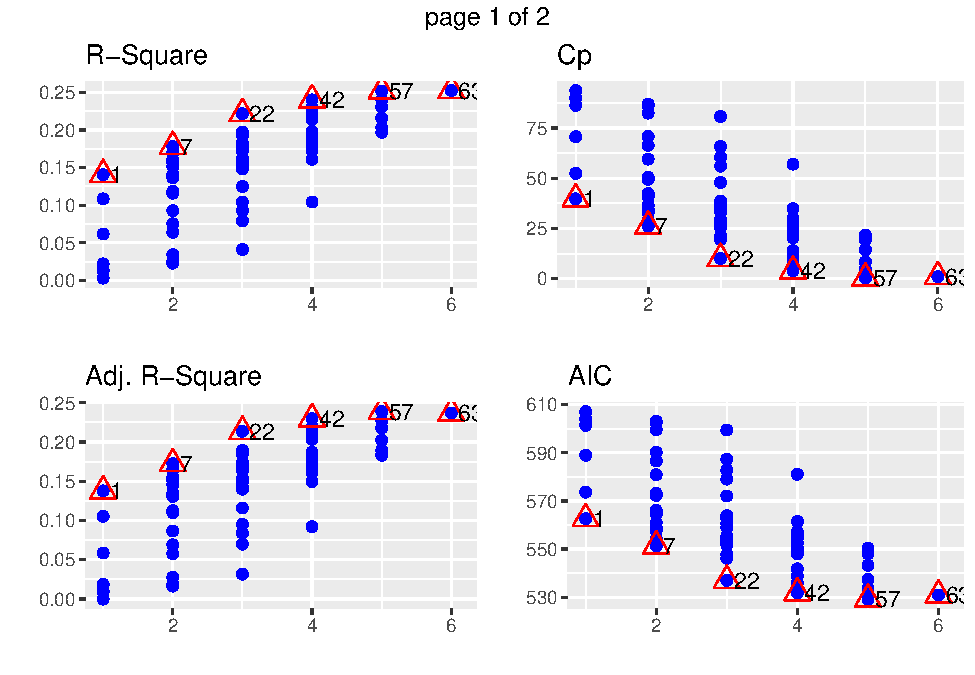
\includegraphics{TP_files/figure-latex/unnamed-chunk-46-1.pdf} Según el
gráfico, el lambda óptimo se encuentra cerca de -1. Entonces
consideraremos la transformación de potencia sobre la variable
respuesta.

\begin{Shaded}
\begin{Highlighting}[]
\CommentTok{\# Se encuentra el valor óptimo de lambda que maximiza el logaritmo de verosimilitud}
\NormalTok{best\_box\_cox }\OtherTok{\textless{}{-}}\NormalTok{ box\_cox\_result}\SpecialCharTok{$}\NormalTok{x[}\FunctionTok{which.max}\NormalTok{(box\_cox\_result}\SpecialCharTok{$}\NormalTok{y)]}

\CommentTok{\# Se ajusta un modelo de regresión lineal utilizando la variable dependiente "Energía" elevada a la potencia óptima de lambda (best\_box\_cox) como la variable de respuesta y la variable independiente "Hora".}
\NormalTok{modelE2 }\OtherTok{\textless{}{-}} \FunctionTok{lm}\NormalTok{((Energía)}\SpecialCharTok{\^{}}\NormalTok{(best\_box\_cox) }\SpecialCharTok{\textasciitilde{}}\NormalTok{ Hora, }\AttributeTok{data =}\NormalTok{ energia)}

\FunctionTok{summary}\NormalTok{(modelE2)}
\end{Highlighting}
\end{Shaded}

\begin{verbatim}
## 
## Call:
## lm(formula = (Energía)^(best_box_cox) ~ Hora, data = energia)
## 
## Residuals:
##        Min         1Q     Median         3Q        Max 
## -1.290e-04 -3.263e-05  3.849e-06  3.599e-05  1.150e-04 
## 
## Coefficients:
##               Estimate Std. Error t value Pr(>|t|)    
## (Intercept)  2.779e-04  1.787e-05   15.55   <2e-16 ***
## Hora        -1.251e-08  6.350e-07   -0.02    0.984    
## ---
## Signif. codes:  0 '***' 0.001 '**' 0.01 '*' 0.05 '.' 0.1 ' ' 1
## 
## Residual standard error: 6.094e-05 on 46 degrees of freedom
## Multiple R-squared:  8.444e-06,  Adjusted R-squared:  -0.02173 
## F-statistic: 0.0003884 on 1 and 46 DF,  p-value: 0.9844
\end{verbatim}

\begin{Shaded}
\begin{Highlighting}[]
\FunctionTok{shapiro.test}\NormalTok{(modelE2}\SpecialCharTok{$}\NormalTok{residuals)}
\end{Highlighting}
\end{Shaded}

\begin{verbatim}
## 
##  Shapiro-Wilk normality test
## 
## data:  modelE2$residuals
## W = 0.98002, p-value = 0.5796
\end{verbatim}

Interpretación:

\begin{itemize}
\item
  El coeficiente del intercepto (Intercept) es 2.779e-04, lo cual
  representa el valor esperado de la variable de respuesta cuando la
  variable predictora es igual a cero. El coeficiente de la variable
  predictora ``Hora'' es -1.251e-08, lo que indica que hay una relación
  muy débil y casi nula entre la variable ``Hora'' y la variable de
  respuesta ``Energía''.
\item
  El coeficiente de determinación (R-cuadrado) múltiple es
  extremadamente bajo, con un valor de 8.444e-06. Esto indica que el
  modelo solo explica una fracción muy pequeña de la variabilidad de los
  datos de la variable de respuesta. El R-cuadrado ajustado tiene un
  valor negativo de -0.02173, lo que sugiere que el modelo no se ajusta
  bien a los datos.
\item
  El valor del estadístico F es de 0.0003884 con un p-value asociado de
  0.9844. Esto indica que el modelo en su conjunto no es
  estadísticamente significativo, lo que sugiere que no hay evidencia
  suficiente para afirmar que el modelo es una mejora significativa
  sobre un modelo nulo.
\item
  La prueba de normalidad de Shapiro-Wilk se utiliza para evaluar si los
  residuos del modelo siguen una distribución normal. En este caso, el
  valor de W obtenido es 0.98002, y el p-value asociado es 0.5796. Como
  el p-value es mayor que 0.05, no hay suficiente evidencia para
  rechazar la hipótesis nula de normalidad de los residuos.
\end{itemize}

En resumen, el modelo ajustado no es capaz de explicar la variabilidad
en los datos de manera satisfactoria, no muestra una relación
significativa entre la variable predictora ``Hora'' y la variable de
respuesta ``Energía'', y los residuos no siguen una distribución normal.

\begin{Shaded}
\begin{Highlighting}[]
\CommentTok{\# Crea una copia}
\NormalTok{energia3}\OtherTok{\textless{}{-}}\NormalTok{energia}

\CommentTok{\# Se calcula el logaritmo natural de la columna "Energía" en el dataframe energia y se asigna a la columna "Energía" en energia3.}
\NormalTok{energia3}\SpecialCharTok{$}\NormalTok{Energía }\OtherTok{\textless{}{-}} \FunctionTok{log}\NormalTok{(energia}\SpecialCharTok{$}\NormalTok{Energía)}

\CommentTok{\# Se agrega una columna llamada "prediccion" en energia3 que contiene los valores ajustados del modelo modelE2.}
\NormalTok{energia3}\SpecialCharTok{$}\NormalTok{prediccion }\OtherTok{\textless{}{-}}\NormalTok{ modelE2}\SpecialCharTok{$}\NormalTok{fitted.values }

\CommentTok{\# Se agrega una columna llamada "residuos" en energia3 que contiene los residuos del modelo modelE2.}
\NormalTok{energia3}\SpecialCharTok{$}\NormalTok{residuos }\OtherTok{\textless{}{-}}\NormalTok{ modelE2}\SpecialCharTok{$}\NormalTok{residuals}

\CommentTok{\# Se crea un gráfico de histograma de los residuos utilizando la librería ggplot. Los residuos se representan en el eje x y la densidad en el eje y.}
\FunctionTok{ggplot}\NormalTok{(}\AttributeTok{data =}\NormalTok{ energia3, }\FunctionTok{aes}\NormalTok{(}\AttributeTok{x =}\NormalTok{ residuos)) }\SpecialCharTok{+} \FunctionTok{geom\_histogram}\NormalTok{(}\FunctionTok{aes}\NormalTok{(}\AttributeTok{y =}\NormalTok{ ..density..)) }\SpecialCharTok{+} 
  \FunctionTok{labs}\NormalTok{(}\AttributeTok{title =} \StringTok{"Histograma de los residuos"}\NormalTok{) }\SpecialCharTok{+} \FunctionTok{theme\_bw}\NormalTok{() }\SpecialCharTok{+} 
  \FunctionTok{theme}\NormalTok{(}\AttributeTok{plot.title =} \FunctionTok{element\_text}\NormalTok{(}\AttributeTok{hjust =} \FloatTok{0.5}\NormalTok{))}
\end{Highlighting}
\end{Shaded}

\begin{verbatim}
## Warning: The dot-dot notation (`..density..`) was deprecated in ggplot2 3.4.0.
## i Please use `after_stat(density)` instead.
## This warning is displayed once every 8 hours.
## Call `lifecycle::last_lifecycle_warnings()` to see where this warning was
## generated.
\end{verbatim}

\begin{verbatim}
## `stat_bin()` using `bins = 30`. Pick better value with `binwidth`.
\end{verbatim}

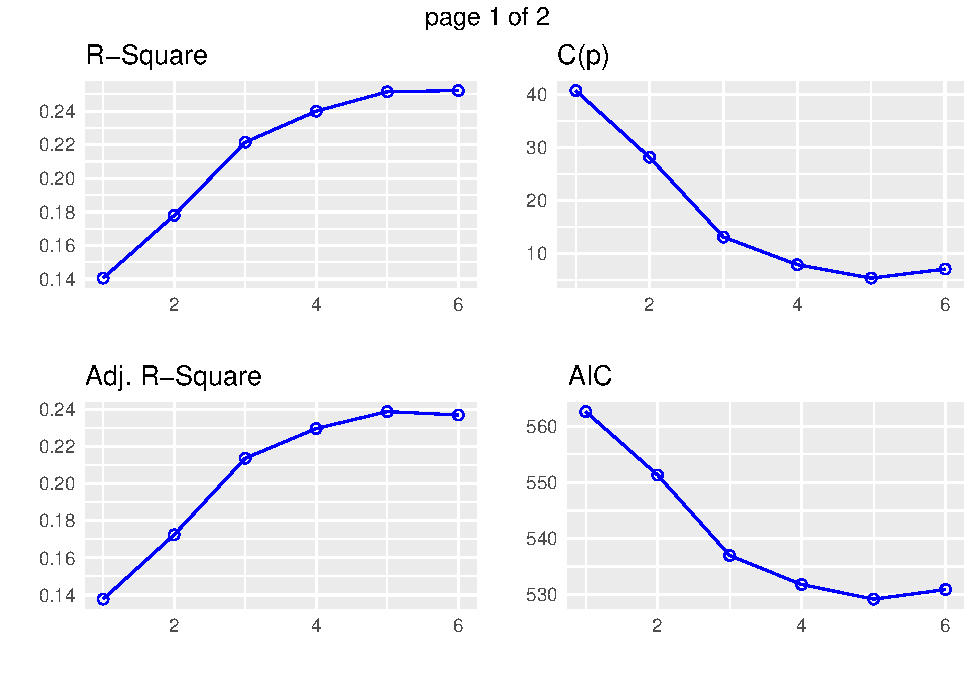
\includegraphics{TP_files/figure-latex/unnamed-chunk-48-1.pdf}

\begin{Shaded}
\begin{Highlighting}[]
\CommentTok{\# Se crea un gráfico de cuantiles normales (QQ plot) de los residuos del modelo modelE2.}
\FunctionTok{qqnorm}\NormalTok{(modelE2}\SpecialCharTok{$}\NormalTok{residuals) }

\CommentTok{\# Se crea una linea de referencia en el grafico}
\FunctionTok{qqline}\NormalTok{(modelE2}\SpecialCharTok{$}\NormalTok{residuals)}
\end{Highlighting}
\end{Shaded}

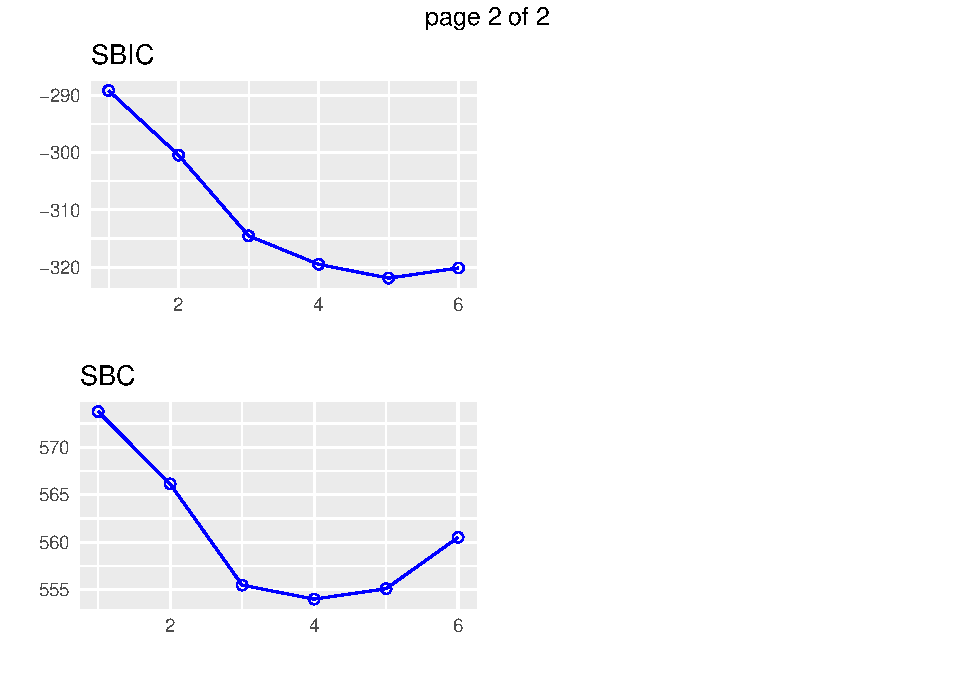
\includegraphics{TP_files/figure-latex/unnamed-chunk-48-2.pdf}

\begin{Shaded}
\begin{Highlighting}[]
\NormalTok{linMod2 }\OtherTok{\textless{}{-}} \FunctionTok{lm}\NormalTok{(}\FunctionTok{log10}\NormalTok{(Energía) }\SpecialCharTok{\textasciitilde{}}\NormalTok{ Hora, }\AttributeTok{data =}\NormalTok{ energia)}
\FunctionTok{summary}\NormalTok{(linMod2)}
\end{Highlighting}
\end{Shaded}

\begin{verbatim}
## 
## Call:
## lm(formula = log10(Energía) ~ Hora, data = energia)
## 
## Residuals:
##      Min       1Q   Median       3Q      Max 
## -0.12212 -0.04859 -0.01411  0.03415  0.19541 
## 
## Coefficients:
##              Estimate Std. Error t value Pr(>|t|)    
## (Intercept) 2.6899875  0.0224064 120.055   <2e-16 ***
## Hora        0.0002440  0.0007961   0.306    0.761    
## ---
## Signif. codes:  0 '***' 0.001 '**' 0.01 '*' 0.05 '.' 0.1 ' ' 1
## 
## Residual standard error: 0.07641 on 46 degrees of freedom
## Multiple R-squared:  0.002038,   Adjusted R-squared:  -0.01966 
## F-statistic: 0.09393 on 1 and 46 DF,  p-value: 0.7606
\end{verbatim}

Los valores de t-value y p-value para el coeficiente de Hora son 0.306 y
0.761 respectivamente. Esto indica que no hay evidencia significativa
para afirmar que la variable Hora tenga un efecto significativo en el
logaritmo en base 10 de la variable Energía.

El R cuadrado múltiple ajustado es de -0.01966, lo que sugiere que el
modelo no explica de manera efectiva la variabilidad en el logaritmo en
base 10 de la variable Energía.

El F-estadístico tiene un valor de 0.09393 y un p-value de 0.7606. Esto
indica que el modelo en su conjunto no es estadísticamente
significativo.

En resumen, los resultados sugieren que el modelo de regresión lineal
con la variable Hora como predictor no es adecuado para explicar la
variabilidad en el logaritmo en base 10 de la variable Energía. No se
encontró una relación significativa entre estas dos variables.

\begin{Shaded}
\begin{Highlighting}[]
\FunctionTok{plot}\NormalTok{(energia}\SpecialCharTok{$}\NormalTok{Hora,}\FunctionTok{log10}\NormalTok{(energia}\SpecialCharTok{$}\NormalTok{Energía),}\AttributeTok{xlab=}\StringTok{"Hora"}\NormalTok{,}\AttributeTok{ylab=}\StringTok{"log10(Energía)"}\NormalTok{,}
     \AttributeTok{main=}\StringTok{"Hora vs log10(Energía)"}\NormalTok{)}

\FunctionTok{abline}\NormalTok{(linMod2,}\AttributeTok{col=}\StringTok{"darkviolet"}\NormalTok{,}\AttributeTok{lwd=}\DecValTok{2}\NormalTok{)}
\end{Highlighting}
\end{Shaded}

\includegraphics{TP_files/figure-latex/unnamed-chunk-50-1.pdf}

\hypertarget{d-2}{%
\subsubsection{(d)}\label{d-2}}

Realizar el análisis diagnóstico del nuevo modelo y estimar un intervalo
de confianza y un intervalo de predicción para 27.5 hs con ambos
modelos. Comparar los intervalos.

análisis diagnóstico

\begin{Shaded}
\begin{Highlighting}[]
\FunctionTok{shapiro.test}\NormalTok{(linMod2}\SpecialCharTok{$}\NormalTok{residuals)}
\end{Highlighting}
\end{Shaded}

\begin{verbatim}
## 
##  Shapiro-Wilk normality test
## 
## data:  linMod2$residuals
## W = 0.96393, p-value = 0.1454
\end{verbatim}

W (estadístico de prueba): El valor de W obtenido es 0.96393. Este valor
se utiliza para evaluar la desviación de la normalidad. Un valor cercano
a 1 indica que los datos se ajustan bien a una distribución normal.

p-value (valor p): El valor p obtenido es 0.1454. Es una medida de la
evidencia en contra de la hipótesis nula de que los residuos siguen una
distribución normal. Un valor p mayor a un umbral (generalmente 0.05)
indica que no hay suficiente evidencia para rechazar la hipótesis nula y
se puede considerar que los residuos se distribuyen aproximadamente de
manera normal.

En este caso, el valor p es 0.1454, lo que sugiere que no hay suficiente
evidencia para rechazar la hipótesis nula de normalidad de los residuos.
Por lo tanto, se puede asumir que los residuos del modelo siguen una
distribución aproximadamente normal.

\begin{Shaded}
\begin{Highlighting}[]
\FunctionTok{library}\NormalTok{(car)}

\CommentTok{\# Prueba de heterocedasticidad }
\FunctionTok{ncvTest}\NormalTok{(modelE2)}
\end{Highlighting}
\end{Shaded}

\begin{verbatim}
## Non-constant Variance Score Test 
## Variance formula: ~ fitted.values 
## Chisquare = 2.758408, Df = 1, p = 0.096744
\end{verbatim}

Dado que el valor p (0.096744) es mayor que el nivel de significancia
comúnmente utilizado (como 0.05), no hay suficiente evidencia para
rechazar la hipótesis nula. Por lo tanto, no se encontró evidencia
suficiente para concluir que hay heterocedasticidad en los residuos del
modelo modelE2. Esto sugiere que la varianza de los residuos es
constante, lo que cumple con la asunción de homocedasticidad en el
modelo lineal.

\begin{Shaded}
\begin{Highlighting}[]
\CommentTok{\#  Prueba de autocorrelación de primer orden utilizando el estadístico de Durbin{-}Watson (D{-}W)}
\FunctionTok{dwt}\NormalTok{(linMod2)}
\end{Highlighting}
\end{Shaded}

\begin{verbatim}
##  lag Autocorrelation D-W Statistic p-value
##    1       0.0159792      1.877106   0.576
##  Alternative hypothesis: rho != 0
\end{verbatim}

El estadístico D-W tiene un rango de valores entre 0 y 4 y se utiliza
para detectar la presencia de autocorrelación en los residuos de un
modelo de regresión.

En este caso, el valor del estadístico D-W es 1.877106. El rango de
valores cercanos a 2 sugiere la ausencia de autocorrelación de primer
orden en los residuos. Sin embargo, para interpretar adecuadamente el
resultado, también se debe considerar el valor p asociado al
estadístico.

El valor p asociado al estadístico D-W es 0.608. Dado que este valor p
es mayor que el nivel de significancia comúnmente utilizado (como 0.05),
no hay suficiente evidencia para rechazar la hipótesis nula de que no
hay autocorrelación de primer orden en los residuos.

En resumen, no se encontró evidencia de autocorrelación de primer orden
en los residuos del modelo modelE2, lo que indica que los residuos están
aproximadamente no correlacionados entre sí.

Aunque se cumplen los supuestos con el modelo \texttt{linMod2}, en
definitiva, utilizando transformaciones no se logra ajustar un modelo de
regresión que cumpla con un R cuadrado suficientemente alto para inferir
que una variable explica la otra.

\begin{Shaded}
\begin{Highlighting}[]
\CommentTok{\# Intervalo de confianza modelo 2}
\NormalTok{ic }\OtherTok{\textless{}{-}} \FunctionTok{confint}\NormalTok{(model14, }\AttributeTok{level =} \FloatTok{0.95}\NormalTok{)}
\NormalTok{ic}
\end{Highlighting}
\end{Shaded}

\begin{verbatim}
##                 2.5 %     97.5 %
## (Intercept) 436.12578 546.852940
## Hora         -1.44621   2.487895
\end{verbatim}

\begin{Shaded}
\begin{Highlighting}[]
\CommentTok{\# Intervalo de confianza modelo 2}
\NormalTok{ic }\OtherTok{\textless{}{-}} \FunctionTok{confint}\NormalTok{(modelE2, }\AttributeTok{level =} \FloatTok{0.95}\NormalTok{)}
\NormalTok{ic}
\end{Highlighting}
\end{Shaded}

\begin{verbatim}
##                     2.5 %       97.5 %
## (Intercept)  2.419201e-04 3.138658e-04
## Hora        -1.290618e-06 1.265591e-06
\end{verbatim}

\begin{Shaded}
\begin{Highlighting}[]
\CommentTok{\# Intervalo de confianza modelo 3}
\NormalTok{ic }\OtherTok{\textless{}{-}} \FunctionTok{confint}\NormalTok{(linMod2, }\AttributeTok{level =} \FloatTok{0.95}\NormalTok{)}
\NormalTok{ic}
\end{Highlighting}
\end{Shaded}

\begin{verbatim}
##                    2.5 %      97.5 %
## (Intercept)  2.644885797 2.735089103
## Hora        -0.001358468 0.001846429
\end{verbatim}

Predicción

\begin{Shaded}
\begin{Highlighting}[]
\NormalTok{ic1}\OtherTok{=}\FunctionTok{predict}\NormalTok{(model14, }\AttributeTok{newdata =} \FunctionTok{data.frame}\NormalTok{(}\AttributeTok{Hora =} \FunctionTok{c}\NormalTok{(}\FloatTok{27.5}\NormalTok{)),}\AttributeTok{interval=}\StringTok{"confidence"}\NormalTok{)}
\NormalTok{ip1}\OtherTok{=}\FunctionTok{predict}\NormalTok{(model14, }\AttributeTok{newdata =} \FunctionTok{data.frame}\NormalTok{(}\AttributeTok{Hora =} \FunctionTok{c}\NormalTok{(}\FloatTok{27.5}\NormalTok{)),}\AttributeTok{interval=}\StringTok{"prediction"}\NormalTok{)}
\NormalTok{ic1}
\end{Highlighting}
\end{Shaded}

\begin{verbatim}
##        fit      lwr      upr
## 1 505.8125 477.9305 533.6945
\end{verbatim}

\begin{Shaded}
\begin{Highlighting}[]
\NormalTok{ip1}
\end{Highlighting}
\end{Shaded}

\begin{verbatim}
##        fit      lwr      upr
## 1 505.8125 314.9688 696.6563
\end{verbatim}

\begin{Shaded}
\begin{Highlighting}[]
\NormalTok{ic2}\OtherTok{=}\FunctionTok{predict}\NormalTok{(modelE2, }\AttributeTok{newdata =} \FunctionTok{data.frame}\NormalTok{(}\AttributeTok{Hora =} \FunctionTok{c}\NormalTok{(}\FloatTok{27.5}\NormalTok{)),}\AttributeTok{interval=}\StringTok{"confidence"}\NormalTok{)}
\NormalTok{ip2}\OtherTok{=}\FunctionTok{predict}\NormalTok{(modelE2, }\AttributeTok{newdata =} \FunctionTok{data.frame}\NormalTok{(}\AttributeTok{Hora =} \FunctionTok{c}\NormalTok{(}\FloatTok{27.5}\NormalTok{)),}\AttributeTok{interval=}\StringTok{"prediction"}\NormalTok{)}
\NormalTok{ic2}
\end{Highlighting}
\end{Shaded}

\begin{verbatim}
##            fit          lwr          upr
## 1 0.0002775488 0.0002594323 0.0002956653
\end{verbatim}

\begin{Shaded}
\begin{Highlighting}[]
\NormalTok{ip2}
\end{Highlighting}
\end{Shaded}

\begin{verbatim}
##            fit          lwr          upr
## 1 0.0002775488 0.0001535469 0.0004015508
\end{verbatim}

\begin{Shaded}
\begin{Highlighting}[]
\NormalTok{ic3}\OtherTok{=}\FunctionTok{predict}\NormalTok{(linMod2, }\AttributeTok{newdata =} \FunctionTok{data.frame}\NormalTok{(}\AttributeTok{Hora =} \FunctionTok{c}\NormalTok{(}\FloatTok{27.5}\NormalTok{)),}\AttributeTok{interval=}\StringTok{"confidence"}\NormalTok{)}
\NormalTok{ip3}\OtherTok{=}\FunctionTok{predict}\NormalTok{(linMod2, }\AttributeTok{newdata =} \FunctionTok{data.frame}\NormalTok{(}\AttributeTok{Hora =} \FunctionTok{c}\NormalTok{(}\FloatTok{27.5}\NormalTok{)),}\AttributeTok{interval=}\StringTok{"prediction"}\NormalTok{)}
\NormalTok{ic3}
\end{Highlighting}
\end{Shaded}

\begin{verbatim}
##        fit      lwr      upr
## 1 2.696697 2.673983 2.719411
\end{verbatim}

\begin{Shaded}
\begin{Highlighting}[]
\NormalTok{ip3}
\end{Highlighting}
\end{Shaded}

\begin{verbatim}
##        fit      lwr      upr
## 1 2.696697 2.541227 2.852167
\end{verbatim}

Si se toma el último modelo que cumplió los supuestos y se retira la
transformación se tiene:

\begin{Shaded}
\begin{Highlighting}[]
\DecValTok{10}\SpecialCharTok{\^{}}\NormalTok{ic3}
\end{Highlighting}
\end{Shaded}

\begin{verbatim}
##        fit      lwr     upr
## 1 497.3898 472.0445 524.096
\end{verbatim}

\begin{Shaded}
\begin{Highlighting}[]
\DecValTok{10}\SpecialCharTok{\^{}}\NormalTok{ip3}
\end{Highlighting}
\end{Shaded}

\begin{verbatim}
##        fit      lwr      upr
## 1 497.3898 347.7179 711.4867
\end{verbatim}

\hypertarget{tratamiento-de-la-heterocedasticidad}{%
\section{\texorpdfstring{{1.4. Tratamiento de la
heterocedasticidad}}{1.4. Tratamiento de la heterocedasticidad}}\label{tratamiento-de-la-heterocedasticidad}}

\hypertarget{ejercicio-1.5.}{%
\subsection{Ejercicio 1.5.}\label{ejercicio-1.5.}}

Se obtuvieron datos históricos del mercado inmobiliario de una ciudad de
Nueva Taipei, en Taiwan. La base es inmobiliaria.xlsx .

Las características son:

\begin{itemize}
\tightlist
\item
  edad: Edad de la propiedad (en años).
\item
  distancia: La distancia a la estación de transporte más cercana (en
  metros).
\item
  negocios: Cantidad de negocios de conveniencia en las cercanías a una
  distancia realizable a pie.
\item
  latitud: Latitud de la ubicación de la propiedad (en grados).
\item
  longitud: Longitud de la ubicación de la propiedad (en grados).
\item
  precio: Precio por metro cuadrado (en miles de dólares)
\end{itemize}

Se quiere investigar si el precio de las propiedades puede ser estimado
en función de alguna de las variables disponibles.

\begin{Shaded}
\begin{Highlighting}[]
\CommentTok{\# se carga la base}
\NormalTok{baseeje15}\OtherTok{=}\StringTok{"C:/Users/Josvaldes/Documents/Maestria/Austral/1ano/regresionAvanzada/TPRegresion/TPRegresion/inmobiliaria.csv"}
\NormalTok{propiedades }\OtherTok{\textless{}{-}} \FunctionTok{read.csv}\NormalTok{(baseeje15,}\AttributeTok{header =} \ConstantTok{TRUE}\NormalTok{, }\AttributeTok{sep =} \StringTok{";"}\NormalTok{)}

\NormalTok{propiedades}
\end{Highlighting}
\end{Shaded}

\begin{verbatim}
##     edad  distancia negocios latitud longitud precio
## 1   32.0   84.87882       10   24.98   121.54   11.5
## 2   19.5  306.59470        9   24.98   121.54   12.8
## 3   13.3  561.98450        5   24.99   121.54   14.3
## 4   13.3  561.98450        5   24.99   121.54   16.6
## 5    5.0  390.56840        5   24.98   121.54   13.1
## 6    7.1 2176.03000        4   24.96   121.51    9.7
## 7   34.5  623.47310        7   24.98   121.54   12.2
## 8   20.1  287.60250        6   24.98   121.54   14.2
## 9   31.7 5512.03800        1   24.95   121.48    5.7
## 10  17.9 1783.18000        3   24.97   121.51    6.7
## 11  34.7  405.21340        1   24.97   121.53   12.5
## 12   0.2  292.99780        6   24.98   121.54   21.2
## 13  17.7  350.85150        1   24.98   121.53   11.3
## 14  16.9  368.13630        8   24.97   121.54   12.8
## 15   1.5   23.48000        7   24.97   121.54   14.5
## 16   4.5 2275.87700        3   24.96   121.51    8.9
## 17  10.5  279.17260        7   24.98   121.55   15.6
## 18  14.7 1360.13900        1   24.95   121.55    7.5
## 19  10.1  279.17260        7   24.98   121.55   14.5
## 20  39.6  480.69770        4   24.97   121.54   11.8
## 21  29.3 1487.86800        2   24.98   121.52    8.2
## 22   3.1  383.86240        5   24.98   121.54   17.0
## 23  10.4  276.44900        4   24.96   121.54   10.2
## 24  19.2  557.47800        5   24.97   121.54   14.2
## 25   7.3  451.24380        5   24.98   121.55   17.3
## 26  25.9 4519.69000        0   24.95   121.50    6.7
## 27  29.6  769.40340        7   24.98   121.53    7.6
## 28  37.9  488.57270        1   24.97   121.53   10.4
## 29  16.5  323.65500        6   24.98   121.54   14.9
## 30  15.4  205.36700        7   24.98   121.54   16.7
## 31  13.9 4079.41800        0   25.01   121.52    8.3
## 32  14.7 1935.00900        2   24.96   121.51    6.9
## 33  12.0 1360.13900        1   24.95   121.55    7.7
## 34   3.1  577.96150        6   24.97   121.55   14.5
## 35  16.2  289.32480        5   24.98   121.54   14.0
## 36  13.6 4082.01500        0   24.94   121.50    4.8
## 37  16.8 4066.58700        0   24.94   121.50    5.5
## 38  36.1  519.46170        5   24.96   121.54   10.5
## 39  34.4  512.78710        6   24.99   121.54   10.3
## 40   2.7  533.47620        4   24.97   121.55   16.3
## 41  36.6  488.81930        8   24.97   121.54   11.6
## 42  21.7  463.96230        9   24.97   121.54   12.7
## 43  35.9  640.73910        3   24.98   121.54   18.6
## 44  24.2 4605.74900        0   24.95   121.50    4.1
## 45  29.4 4510.35900        1   24.95   121.50    4.0
## 46  21.7  512.54870        4   24.97   121.54   13.4
## 47  31.3 1758.40600        1   24.95   121.55    6.3
## 48  32.1 1438.57900        3   24.97   121.52    8.2
## 49  13.3  492.23130        5   24.97   121.54   11.8
## 50  16.1  289.32480        5   24.98   121.54   15.7
## 51  31.7 1160.63200        0   24.95   121.53    4.2
## 52  33.6  371.24950        8   24.97   121.54   12.7
## 53   3.5   56.47425        7   24.96   121.54   16.2
## 54  30.3 4510.35900        1   24.95   121.50    6.8
## 55  13.3  336.05320        5   24.96   121.53   12.8
## 56  11.0 1931.20700        2   24.96   121.51    6.5
## 57   5.3  259.66070        6   24.98   121.55   19.2
## 58  17.2 2175.87700        3   24.96   121.51    8.4
## 59   2.6  533.47620        4   24.97   121.55   16.7
## 60  17.5  995.75540        0   24.96   121.55    7.7
## 61  40.1  123.74290        8   24.98   121.54   13.4
## 62   1.0  193.58450        6   24.97   121.54   15.4
## 63   8.5  104.81010        5   24.97   121.54   17.2
## 64  30.4  464.22300        6   24.98   121.54   11.0
## 65  12.5  561.98450        5   24.99   121.54   12.7
## 66   6.6   90.45606        9   24.97   121.54   17.9
## 67  35.5  640.73910        3   24.98   121.54   12.4
## 68  32.5  424.54420        8   24.98   121.54   11.0
## 69  13.8 4082.01500        0   24.94   121.50    6.1
## 70   6.8  379.55750       10   24.98   121.54   16.5
## 71  12.3 1360.13900        1   24.95   121.55    8.9
## 72  35.9  616.40040        3   24.98   121.54   11.2
## 73  20.5 2185.12800        3   24.96   121.51    7.8
## 74  38.2  552.43710        2   24.98   121.53    9.0
## 75  18.0 1414.83700        1   24.95   121.55    8.0
## 76  11.8  533.47620        4   24.97   121.55   12.2
## 77  30.8  377.79560        6   24.96   121.54   11.2
## 78  13.2  150.93470        7   24.97   121.54   14.6
## 79  25.3 2707.39200        3   24.96   121.51    5.4
## 80  15.1  383.28050        7   24.97   121.54   13.2
## 81   0.0  338.96790        9   24.97   121.54   15.4
## 82   1.8 1455.79800        1   24.95   121.55    8.2
## 83  16.9 4066.58700        0   24.94   121.50    5.5
## 84   8.9 1406.43000        0   24.99   121.53   14.5
## 85  23.0 3947.94500        0   24.95   121.50    7.7
## 86   0.0  274.01440        1   24.97   121.53   13.8
## 87   9.1 1402.01600        0   24.99   121.53   13.1
## 88  20.6 2469.64500        4   24.96   121.51    6.6
## 89  31.9 1146.32900        0   24.95   121.53    4.9
## 90  40.9  167.59890        5   24.97   121.54   12.4
## 91   8.0  104.81010        5   24.97   121.54   15.7
## 92   6.4   90.45606        9   24.97   121.54   18.0
## 93  28.4  617.44240        3   24.98   121.53   10.5
## 94  16.4  289.32480        5   24.98   121.54   15.5
## 95   6.4   90.45606        9   24.97   121.54   18.8
## 96  17.5  964.74960        4   24.99   121.53   11.6
## 97  12.7  170.12890        1   24.97   121.53   10.0
## 98   1.1  193.58450        6   24.97   121.54   16.5
## 99   0.0  208.39050        6   24.96   121.54   13.8
## 100 32.7  392.44590        6   24.96   121.54    9.2
## 101  0.0  292.99780        6   24.98   121.54   21.5
## 102 17.2  189.51810        8   24.98   121.54   14.3
## 103 12.2 1360.13900        1   24.95   121.55    8.1
## 104 31.4  592.50060        2   24.97   121.54   10.3
## 105  4.0 2147.37600        3   24.96   121.51    8.6
## 106  8.1  104.81010        5   24.97   121.54   15.6
## 107 33.3  196.61720        7   24.98   121.54   11.9
## 108  9.9 2102.42700        3   24.96   121.51    7.0
## 109 14.8  393.26060        6   24.96   121.54    2.3
## 110 30.6  143.83830        8   24.98   121.54   16.2
## 111 20.6  737.91610        2   24.98   121.55   14.1
## 112 30.9 6396.28300        1   24.94   121.48    3.7
## 113 13.6 4197.34900        0   24.94   121.50    3.9
## 114 25.3 1583.72200        3   24.97   121.52    9.3
## 115 16.6  289.32480        5   24.98   121.54   18.1
## 116 13.3  492.23130        5   24.97   121.54    9.5
## 117 13.6  492.23130        5   24.97   121.54   14.5
## 118 31.5  414.94760        4   24.98   121.54    9.8
## 119  0.0  185.42960        0   24.97   121.53   13.8
## 120  9.9  279.17260        7   24.98   121.55   17.4
## 121  1.1  193.58450        6   24.97   121.54   14.7
## 122 38.6  804.68970        4   24.98   121.53   19.1
## 123  3.8  383.86240        5   24.98   121.54   16.7
## 124 41.3  124.99120        6   24.97   121.54   18.4
## 125 38.5  216.83290        7   24.98   121.54   12.4
## 126 29.6  535.52700        8   24.98   121.54   11.4
## 127  4.0 2147.37600        3   24.96   121.51    9.3
## 128 26.6  482.75810        5   24.97   121.54   11.4
## 129 18.0  373.39370        8   24.99   121.54   12.0
## 130 33.4  186.96860        6   24.97   121.54   12.8
## 131 18.9 1009.23500        0   24.96   121.55    6.3
## 132 11.4  390.56840        5   24.98   121.54   14.2
## 133 13.6  319.07080        6   24.96   121.54   14.4
## 134 10.0  942.46640        0   24.98   121.52   13.2
## 135 12.9  492.23130        5   24.97   121.54   12.9
## 136 16.2  289.32480        5   24.98   121.54   15.6
## 137  5.1 1559.82700        3   24.97   121.52    8.8
## 138 19.8  640.60710        5   24.97   121.55   11.4
## 139 13.6  492.23130        5   24.97   121.54   12.2
## 140 11.9 1360.13900        1   24.95   121.55    8.6
## 141  2.1  451.24380        5   24.98   121.55   13.8
## 142  0.0  185.42960        0   24.97   121.53   15.8
## 143  3.2  489.88210        8   24.97   121.54   13.1
## 144 16.4 3780.59000        0   24.93   121.51   13.7
## 145 34.9  179.45380        8   24.97   121.54   12.0
## 146 35.8  170.73110        7   24.97   121.54   14.7
## 147  4.9  387.77210        9   24.98   121.54   13.5
## 148 12.0 1360.13900        1   24.95   121.55    8.8
## 149  6.5  376.17090        6   24.95   121.54   12.4
## 150 16.9 4066.58700        0   24.94   121.50    6.3
## 151 13.8 4082.01500        0   24.94   121.50    4.7
## 152 30.7 1264.73000        0   24.95   121.53    5.5
## 153 16.1  815.93140        4   24.98   121.53   10.8
## 154 11.6  390.56840        5   24.98   121.54   11.9
## 155 15.5  815.93140        4   24.98   121.53   11.3
## 156  3.5   49.66105        8   24.96   121.54   17.5
## 157 19.2  616.40040        3   24.98   121.54   12.0
## 158 16.0 4066.58700        0   24.94   121.50    3.5
## 159  8.5  104.81010        5   24.97   121.54   16.8
## 160  0.0  185.42960        0   24.97   121.53   16.7
## 161 13.7 1236.56400        1   24.98   121.55    9.3
## 162  0.0  292.99780        6   24.98   121.54   22.3
## 163 28.2  330.08540        8   24.97   121.54   13.2
## 164 27.6  515.11220        5   24.96   121.54   11.3
## 165  8.4 1962.62800        1   24.95   121.55    7.1
## 166 24.0 4527.68700        0   24.95   121.50    4.4
## 167  3.6  383.86240        5   24.98   121.54   17.8
## 168  6.6   90.45606        9   24.97   121.54   17.6
## 169 41.3  401.88070        4   24.98   121.54   10.6
## 170  4.3  432.03850        7   24.98   121.54   13.7
## 171 30.2  472.17450        3   24.97   121.54   11.1
## 172 13.9 4573.77900        0   24.95   121.50    5.8
## 173 33.0  181.07660        9   24.98   121.54   12.7
## 174 13.1 1144.43600        4   24.99   121.53   11.1
## 175 14.0  438.85130        1   24.97   121.53   12.9
## 176 26.9 4449.27000        0   24.95   121.50    4.7
## 177 11.6  201.89390        8   24.98   121.54   16.9
## 178 13.5 2147.37600        3   24.96   121.51    7.2
## 179 17.0 4082.01500        0   24.94   121.50    5.7
## 180 14.1 2615.46500        0   24.95   121.56    6.6
## 181 31.4 1447.28600        3   24.97   121.52    6.5
## 182 20.9 2185.12800        3   24.96   121.51    7.8
## 183  8.9 3078.17600        0   24.95   121.57    6.7
## 184 34.8  190.03920        8   24.98   121.54   13.4
## 185 16.3 4066.58700        0   24.94   121.50    6.2
## 186 35.3  616.57350        8   24.98   121.54   12.8
## 187 13.2  750.07040        2   24.97   121.55   11.5
## 188 43.8   57.58945        7   24.97   121.54   12.9
## 189  9.7  421.47900        5   24.98   121.54   14.9
## 190 15.2 3771.89500        0   24.93   121.51    8.9
## 191 15.2  461.10160        5   24.95   121.54   10.5
## 192 22.8  707.90670        2   24.98   121.55   11.1
## 193 34.4  126.72860        8   24.97   121.54   14.6
## 194 34.0  157.60520        7   24.97   121.54   11.8
## 195 18.2  451.64190        8   24.97   121.54    9.6
## 196 17.4  995.75540        0   24.96   121.55    7.7
## 197 13.1  561.98450        5   24.99   121.54   13.9
## 198 38.3  642.69850        3   24.98   121.54    9.5
## 199 15.6  289.32480        5   24.98   121.54   14.0
## 200 18.0 1414.83700        1   24.95   121.55    8.1
## 201 12.8 1449.72200        3   24.97   121.52    6.5
## 202 22.2  379.55750       10   24.98   121.54   13.3
## 203 38.5  665.06360        3   24.98   121.54   10.4
## 204 11.5 1360.13900        1   24.95   121.55    7.9
## 205 34.8  175.62940        8   24.97   121.54   12.4
## 206  5.2  390.56840        5   24.98   121.54   15.8
## 207  0.0  274.01440        1   24.97   121.53   13.2
## 208 17.6 1805.66500        2   24.99   121.52    9.4
## 209  6.2   90.45606        9   24.97   121.54   17.6
## 210 18.1 1783.18000        3   24.97   121.51    6.3
## 211 19.2  383.71290        8   24.97   121.54   14.6
## 212 37.8  590.92920        1   24.97   121.54   12.0
## 213 28.0  372.62420        6   24.98   121.54   12.4
## 214 13.6  492.23130        5   24.97   121.54   13.3
## 215 29.3  529.77710        8   24.98   121.54   12.2
## 216 37.2  186.51010        9   24.98   121.54   23.7
## 217  9.0 1402.01600        0   24.99   121.53   11.7
## 218 30.6  431.11140       10   24.98   121.54   14.7
## 219  9.1 1402.01600        0   24.99   121.53   12.8
## 220 34.5  324.94190        6   24.98   121.54   13.9
## 221  1.1  193.58450        6   24.97   121.54   14.8
## 222 16.5 4082.01500        0   24.94   121.50    3.9
## 223 32.4  265.06090        8   24.98   121.54   12.2
## 224 11.9 3171.32900        0   25.00   121.52   14.1
## 225 31.0 1156.41200        0   24.95   121.53    5.8
## 226  4.0 2147.37600        3   24.96   121.51   10.1
## 227 16.2 4074.73600        0   24.94   121.50    4.5
## 228 27.1 4412.76500        1   24.95   121.50    5.3
## 229 39.7  333.36790        9   24.98   121.54    9.8
## 230  8.0 2216.61200        4   24.96   121.51    7.2
## 231 12.9  250.63100        7   24.97   121.54   11.9
## 232  3.6  373.83890       10   24.98   121.54   18.8
## 233 13.0  732.85280        0   24.98   121.53   11.8
## 234 12.8  732.85280        0   24.98   121.53   12.3
## 235 18.1  837.72330        0   24.96   121.55    9.0
## 236 11.0 1712.63200        2   24.96   121.52    8.7
## 237 13.7  250.63100        7   24.97   121.54   12.5
## 238  2.0 2077.39000        3   24.96   121.51   10.1
## 239 32.8  204.17050        8   24.98   121.54   14.6
## 240  4.8 1559.82700        3   24.97   121.52    6.6
## 241  7.5  639.61980        5   24.97   121.55   12.4
## 242 16.4  389.82190        6   24.96   121.54   12.3
## 243 21.7 1055.06700        0   24.96   121.55    7.0
## 244 19.0 1009.23500        0   24.96   121.55    6.8
## 245 18.0 6306.15300        1   24.96   121.48    4.5
## 246 39.2  424.71320        7   24.97   121.54    9.1
## 247 31.7 1159.45400        0   24.95   121.53    4.2
## 248  5.9   90.45606        9   24.97   121.54   16.0
## 249 30.4 1735.59500        2   24.96   121.52    7.8
## 250  1.1  329.97470        5   24.98   121.54   15.7
## 251 31.5 5512.03800        1   24.95   121.48    5.3
## 252 14.6  339.22890        1   24.98   121.53    8.0
## 253 17.3  444.13340        1   24.98   121.53   13.3
## 254  0.0  292.99780        6   24.98   121.54   19.2
## 255 17.7  837.72330        0   24.96   121.55    8.7
## 256 17.0 1485.09700        4   24.97   121.52    9.3
## 257 16.2 2288.01100        3   24.96   121.51    7.4
## 258 15.9  289.32480        5   24.98   121.54   16.1
## 259  3.9 2147.37600        3   24.96   121.51    9.6
## 260 32.6  493.65700        7   24.97   121.55   12.3
## 261 15.7  815.93140        4   24.98   121.53   11.5
## 262 17.8 1783.18000        3   24.97   121.51    7.2
## 263 34.7  482.75810        5   24.97   121.54   12.5
## 264 17.2  390.56840        5   24.98   121.54   12.2
## 265 17.6  837.72330        0   24.96   121.55    7.0
## 266 10.8  252.58220        1   24.97   121.53   35.6
## 267 17.7  451.64190        8   24.97   121.54    8.0
## 268 13.0  492.23130        5   24.97   121.54   12.3
## 269 13.2  170.12890        1   24.97   121.53    8.9
## 270 27.5  394.01730        7   24.97   121.54   12.4
## 271  1.5   23.38284        7   24.97   121.54   15.1
## 272 19.1  461.10160        5   24.95   121.54   10.3
## 273 21.2 2185.12800        3   24.96   121.51    8.4
## 274  0.0  208.39050        6   24.96   121.54   13.3
## 275  2.6 1554.25000        3   24.97   121.52    9.4
## 276  2.3  184.33020        6   24.97   121.54   13.8
## 277  4.7  387.77210        9   24.98   121.54   13.6
## 278  2.0 1455.79800        1   24.95   121.55    7.8
## 279 33.5 1978.67100        2   24.99   121.52    7.1
## 280 15.0  383.28050        7   24.97   121.54   10.4
## 281 30.1  718.29370        3   24.98   121.54   16.8
## 282  5.9   90.45606        9   24.97   121.54   17.1
## 283 19.2  461.10160        5   24.95   121.54   10.0
## 284 16.6  323.69120        6   24.98   121.54   15.5
## 285 13.9  289.32480        5   24.98   121.54   13.5
## 286 37.7  490.34460        0   24.97   121.53   11.2
## 287  3.4   56.47425        7   24.96   121.54   16.5
## 288 17.5  395.67470        5   24.96   121.53    7.4
## 289 12.6  383.28050        7   24.97   121.54   12.9
## 290 26.4  335.52730        6   24.98   121.54   11.5
## 291 18.2 2179.59000        3   24.96   121.51    6.6
## 292 12.5 1144.43600        4   24.99   121.53   10.3
## 293 34.9  567.03490        4   24.97   121.55    8.6
## 294 16.7 4082.01500        0   24.94   121.50    5.1
## 295 33.2  121.72620       10   24.98   121.54   14.0
## 296  2.5  156.24420        4   24.97   121.54   11.2
## 297 38.0  461.78480        0   24.97   121.53   10.8
## 298 16.5 2288.01100        3   24.96   121.51    7.0
## 299 38.3  439.71050        0   24.97   121.53   11.6
## 300 20.0 1626.08300        3   24.97   121.52    8.9
## 301 16.2  289.32480        5   24.98   121.54   16.7
## 302 14.4  169.98030        1   24.97   121.53   15.2
## 303 10.3 3079.89000        0   24.95   121.57    7.5
## 304 16.4  289.32480        5   24.98   121.54   16.1
## 305 30.3 1264.73000        0   24.95   121.53    5.8
## 306 16.4 1643.49900        2   24.95   121.55    7.5
## 307 21.3  537.79710        4   24.97   121.54   12.8
## 308 35.4  318.52920        9   24.97   121.54   23.6
## 309  8.3  104.81010        5   24.97   121.54   13.0
## 310  3.7  577.96150        6   24.97   121.55   12.6
## 311 15.6 1756.41100        2   24.98   121.52    8.3
## 312 13.3  250.63100        7   24.97   121.54   12.7
## 313 15.6  752.76690        2   24.98   121.53   11.4
## 314  7.1  379.55750       10   24.98   121.54   15.1
## 315 34.6  272.67830        5   24.96   121.54    8.2
## 316 13.5 4197.34900        0   24.94   121.50    5.6
## 317 16.9  964.74960        4   24.99   121.53   11.4
## 318 12.9  187.48230        1   24.97   121.53   10.0
## 319 28.6  197.13380        6   24.98   121.54   12.9
## 320 12.4 1712.63200        2   24.96   121.52    9.5
## 321 36.6  488.81930        8   24.97   121.54   11.5
## 322  4.1   56.47425        7   24.96   121.54   18.8
## 323  3.5  757.33770        3   24.98   121.55   11.1
## 324 15.9 1497.71300        3   24.97   121.52    7.2
## 325 13.6 4197.34900        0   24.94   121.50    5.8
## 326 32.0 1156.77700        0   24.95   121.53    3.9
## 327 25.6 4519.69000        0   24.95   121.50    4.7
## 328 39.8  617.71340        2   24.98   121.53   12.0
## 329  7.8  104.81010        5   24.97   121.54   11.6
## 330 30.0 1013.34100        5   24.99   121.53    6.9
## 331 27.3  337.60160        6   24.96   121.54   11.1
## 332  5.1 1867.23300        2   24.98   121.52   10.8
## 333 31.3  600.86040        5   24.97   121.55    9.4
## 334 31.5  258.18600        9   24.97   121.54   11.0
## 335  1.7  329.97470        5   24.98   121.54   15.3
## 336 33.6  270.88950        0   24.97   121.53   13.0
## 337 13.0  750.07040        2   24.97   121.55   11.2
## 338  5.7   90.45606        9   24.97   121.54   16.2
## 339 33.5  563.28540        8   24.98   121.54   14.1
## 340 34.6 3085.17000        0   25.00   121.52   12.5
## 341  0.0  185.42960        0   24.97   121.53   11.5
## 342 13.2 1712.63200        2   24.96   121.52    9.3
## 343 17.4 6488.02100        1   24.96   121.47    3.4
## 344  4.6  259.66070        6   24.98   121.55   16.3
## 345  7.8  104.81010        5   24.97   121.54   14.2
## 346 13.2  492.23130        5   24.97   121.54   12.8
## 347  4.0 2180.24500        3   24.96   121.51    8.7
## 348 18.4 2674.96100        3   24.96   121.51    7.8
## 349  4.1 2147.37600        3   24.96   121.51    9.5
## 350 12.2 1360.13900        1   24.95   121.55    9.1
## 351  3.8  383.86240        5   24.98   121.54   18.4
## 352 10.3  211.44730        1   24.97   121.53   13.7
## 353  0.0  338.96790        9   24.97   121.54   13.6
## 354  1.1  193.58450        6   24.97   121.54   13.7
## 355  5.6 2408.99300        0   24.96   121.56    7.5
## 356 32.9   87.30222       10   24.98   121.54   14.3
## 357 41.4  281.20500        8   24.97   121.54   19.2
## 358 17.1  967.40000        4   24.99   121.53   12.1
## 359 32.3  109.94550       10   24.98   121.54   14.5
## 360 35.3  614.13940        7   24.98   121.54   10.0
## 361 17.3 2261.43200        4   24.96   121.51    8.9
## 362 14.2 1801.54400        1   24.95   121.55    7.5
## 363 15.0 1828.31900        2   24.96   121.52    6.3
## 364 18.2  350.85150        1   24.98   121.53   13.1
## 365 20.2 2185.12800        3   24.96   121.51    6.9
## 366 15.9  289.32480        5   24.98   121.54   12.8
## 367  4.1  312.89630        5   24.96   121.54   15.7
## 368 33.9  157.60520        7   24.97   121.54   12.6
## 369  0.0  274.01440        1   24.97   121.53   15.8
## 370  5.4  390.56840        5   24.98   121.54   15.0
## 371 21.7 1157.98800        0   24.96   121.55    7.2
## 372 14.7 1717.19300        2   24.96   121.52    9.2
## 373  3.9   49.66105        8   24.96   121.54   17.2
## 374 37.3  587.88770        8   24.97   121.55   11.3
## 375  0.0  292.99780        6   24.98   121.54   21.1
## 376 14.1  289.32480        5   24.98   121.54   16.2
## 377  8.0  132.54690        9   24.98   121.54   14.3
## 378 16.3 3529.56400        0   24.93   121.52    8.9
## 379 29.1  506.11440        4   24.98   121.54   12.2
## 380 16.1 4066.58700        0   24.94   121.50    3.9
## 381 18.3   82.88643       10   24.98   121.54   14.1
## 382  0.0  185.42960        0   24.97   121.53   16.8
## 383 16.2 2103.55500        3   24.96   121.51    7.8
## 384 10.4 2251.93800        4   24.96   121.51    8.3
## 385 40.9  122.36190        8   24.97   121.54   20.5
## 386 32.8  377.83020        9   24.97   121.54   11.7
## 387  6.2 1939.74900        1   24.95   121.55    9.5
## 388 42.7  443.80200        6   24.98   121.54   10.7
## 389 16.9  967.40000        4   24.99   121.53   12.2
## 390 32.6 4136.27100        1   24.96   121.50    7.5
## 391 21.2  512.54870        4   24.97   121.54   12.9
## 392 37.1  918.63570        1   24.97   121.55    9.7
## 393 13.1 1164.83800        4   24.99   121.53    9.8
## 394 14.7 1717.19300        2   24.96   121.52    7.0
## 395 12.7  170.12890        1   24.97   121.53   11.3
## 396 26.8  482.75810        5   24.97   121.54   10.8
## 397  7.6 2175.03000        3   24.96   121.51    8.4
## 398 12.7  187.48230        1   24.97   121.53    8.6
## 399 30.9  161.94200        9   24.98   121.54   12.0
## 400 16.4  289.32480        5   24.98   121.54   12.5
## 401 23.0  130.99450        6   24.96   121.54   11.3
## 402  1.9  372.13860        7   24.97   121.54   12.3
## 403  5.2 2408.99300        0   24.96   121.56    6.8
## 404 18.5 2175.74400        3   24.96   121.51    8.5
## 405 13.7 4082.01500        0   24.94   121.50    4.7
## 406  5.6   90.45606        9   24.97   121.54   15.2
## 407 18.8  390.96960        7   24.98   121.54   12.3
## 408  8.1  104.81010        5   24.97   121.54   15.9
## 409  6.5   90.45606        9   24.97   121.54   19.4
\end{verbatim}

\hypertarget{a-4}{%
\subsubsection{(a)}\label{a-4}}

Analizar si el precio depende de alguna de las variables.

\begin{Shaded}
\begin{Highlighting}[]
\CommentTok{\# Se crea el promedio de las variables}
\NormalTok{promediosP }\OtherTok{\textless{}{-}} \FunctionTok{colMeans}\NormalTok{(propiedades)}

\CommentTok{\# Se crea las graficas }
\CommentTok{\# grafica edad vs precio}
\NormalTok{c1 }\OtherTok{\textless{}{-}} \FunctionTok{ggplot}\NormalTok{(propiedades, }\FunctionTok{aes}\NormalTok{(edad, precio)) }\SpecialCharTok{+} 
  \FunctionTok{geom\_point}\NormalTok{() }\SpecialCharTok{+}
  \FunctionTok{geom\_vline}\NormalTok{(}\AttributeTok{xintercept=}\NormalTok{promediosP[}\DecValTok{1}\NormalTok{],}\AttributeTok{linetype=}\StringTok{"dotted"}\NormalTok{) }\SpecialCharTok{+} 
  \FunctionTok{geom\_hline}\NormalTok{(}\AttributeTok{yintercept=}\NormalTok{promediosP[}\DecValTok{6}\NormalTok{],}\AttributeTok{linetype=}\StringTok{"dotted"}\NormalTok{) }\SpecialCharTok{+}
   \FunctionTok{geom\_smooth}\NormalTok{(}\AttributeTok{method =} \StringTok{"lm"}\NormalTok{, }\AttributeTok{se =} \ConstantTok{TRUE}\NormalTok{, }\AttributeTok{color =} \StringTok{"black"}\NormalTok{) }\SpecialCharTok{+}
  \FunctionTok{theme\_minimal}\NormalTok{()}

\CommentTok{\# grafica distancia vs precio}
\NormalTok{c2 }\OtherTok{\textless{}{-}} \FunctionTok{ggplot}\NormalTok{(propiedades, }\FunctionTok{aes}\NormalTok{(distancia, precio)) }\SpecialCharTok{+} 
  \FunctionTok{geom\_point}\NormalTok{() }\SpecialCharTok{+} 
  \FunctionTok{geom\_vline}\NormalTok{(}\AttributeTok{xintercept=}\NormalTok{promediosP[}\DecValTok{2}\NormalTok{],}\AttributeTok{linetype=}\StringTok{"dotted"}\NormalTok{) }\SpecialCharTok{+}
  \FunctionTok{geom\_hline}\NormalTok{(}\AttributeTok{yintercept=}\NormalTok{promediosP[}\DecValTok{6}\NormalTok{],}\AttributeTok{linetype=}\StringTok{"dotted"}\NormalTok{) }\SpecialCharTok{+} 
   \FunctionTok{geom\_smooth}\NormalTok{(}\AttributeTok{method =} \StringTok{"lm"}\NormalTok{, }\AttributeTok{se =} \ConstantTok{TRUE}\NormalTok{, }\AttributeTok{color =} \StringTok{"black"}\NormalTok{) }\SpecialCharTok{+}
  \FunctionTok{theme\_minimal}\NormalTok{()}

\CommentTok{\# grafica negocios vs precio}
\NormalTok{c3 }\OtherTok{\textless{}{-}} \FunctionTok{ggplot}\NormalTok{(propiedades, }\FunctionTok{aes}\NormalTok{(negocios, precio)) }\SpecialCharTok{+} 
  \FunctionTok{geom\_point}\NormalTok{() }\SpecialCharTok{+}
  \FunctionTok{geom\_vline}\NormalTok{(}\AttributeTok{xintercept=}\NormalTok{promediosP[}\DecValTok{3}\NormalTok{],}\AttributeTok{linetype=}\StringTok{"dotted"}\NormalTok{) }\SpecialCharTok{+} 
  \FunctionTok{geom\_hline}\NormalTok{(}\AttributeTok{yintercept=}\NormalTok{promediosP[}\DecValTok{6}\NormalTok{],}\AttributeTok{linetype=}\StringTok{"dotted"}\NormalTok{) }\SpecialCharTok{+} 
   \FunctionTok{geom\_smooth}\NormalTok{(}\AttributeTok{method =} \StringTok{"lm"}\NormalTok{, }\AttributeTok{se =} \ConstantTok{TRUE}\NormalTok{, }\AttributeTok{color =} \StringTok{"black"}\NormalTok{) }\SpecialCharTok{+}
  \FunctionTok{theme\_minimal}\NormalTok{()}

\CommentTok{\# grafica negocios vs precio}

\NormalTok{c4 }\OtherTok{\textless{}{-}} \FunctionTok{ggplot}\NormalTok{(propiedades, }\FunctionTok{aes}\NormalTok{(latitud, precio)) }\SpecialCharTok{+} 
  \FunctionTok{geom\_point}\NormalTok{() }\SpecialCharTok{+}
  \FunctionTok{geom\_vline}\NormalTok{(}\AttributeTok{xintercept=}\NormalTok{promediosP[}\DecValTok{4}\NormalTok{],}\AttributeTok{linetype=}\StringTok{"dotted"}\NormalTok{) }\SpecialCharTok{+} 
  \FunctionTok{geom\_hline}\NormalTok{(}\AttributeTok{yintercept=}\NormalTok{promediosP[}\DecValTok{6}\NormalTok{],}\AttributeTok{linetype=}\StringTok{"dotted"}\NormalTok{) }\SpecialCharTok{+} 
   \FunctionTok{geom\_smooth}\NormalTok{(}\AttributeTok{method =} \StringTok{"lm"}\NormalTok{, }\AttributeTok{se =} \ConstantTok{TRUE}\NormalTok{, }\AttributeTok{color =} \StringTok{"black"}\NormalTok{) }\SpecialCharTok{+}
  \FunctionTok{theme\_minimal}\NormalTok{()}

\CommentTok{\# grafica longitud vs precio}

\NormalTok{c5 }\OtherTok{\textless{}{-}} \FunctionTok{ggplot}\NormalTok{(propiedades, }\FunctionTok{aes}\NormalTok{(longitud, precio)) }\SpecialCharTok{+} 
  \FunctionTok{geom\_point}\NormalTok{() }\SpecialCharTok{+}
  \FunctionTok{geom\_vline}\NormalTok{(}\AttributeTok{xintercept=}\NormalTok{promediosP[}\DecValTok{5}\NormalTok{],}\AttributeTok{linetype=}\StringTok{"dotted"}\NormalTok{) }\SpecialCharTok{+} 
  \FunctionTok{geom\_hline}\NormalTok{(}\AttributeTok{yintercept=}\NormalTok{promediosP[}\DecValTok{6}\NormalTok{],}\AttributeTok{linetype=}\StringTok{"dotted"}\NormalTok{) }\SpecialCharTok{+} 
   \FunctionTok{geom\_smooth}\NormalTok{(}\AttributeTok{method =} \StringTok{"lm"}\NormalTok{, }\AttributeTok{se =} \ConstantTok{TRUE}\NormalTok{, }\AttributeTok{color =} \StringTok{"black"}\NormalTok{) }\SpecialCharTok{+}
  \FunctionTok{theme\_minimal}\NormalTok{()}

\FunctionTok{grid.arrange}\NormalTok{(c1,c2,c3,c4,c5, }\AttributeTok{ncol =} \DecValTok{3}\NormalTok{, }\AttributeTok{nrow =} \DecValTok{2}\NormalTok{)}
\end{Highlighting}
\end{Shaded}

\begin{verbatim}
## `geom_smooth()` using formula = 'y ~ x'
## `geom_smooth()` using formula = 'y ~ x'
## `geom_smooth()` using formula = 'y ~ x'
## `geom_smooth()` using formula = 'y ~ x'
## `geom_smooth()` using formula = 'y ~ x'
\end{verbatim}

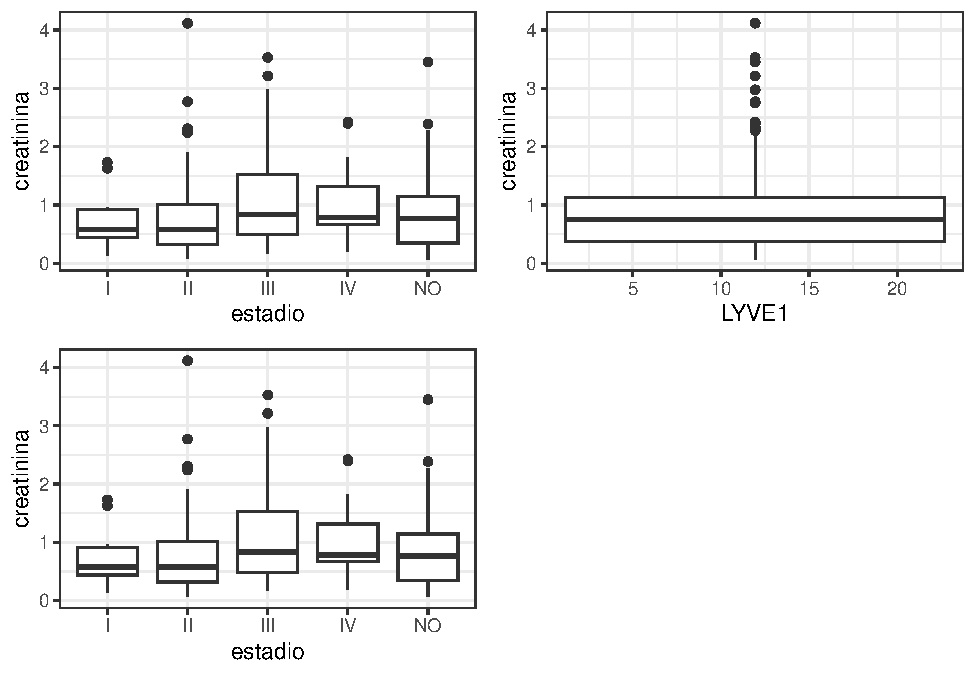
\includegraphics{TP_files/figure-latex/unnamed-chunk-62-1.pdf}

Se realizan los tests:

\begin{Shaded}
\begin{Highlighting}[]
\CommentTok{\# test Precio y edad}
\NormalTok{biNormTest }\OtherTok{\textless{}{-}} \FunctionTok{mvn}\NormalTok{(}\AttributeTok{data =}\NormalTok{ propiedades[}\FunctionTok{c}\NormalTok{(}\DecValTok{6}\NormalTok{,}\DecValTok{1}\NormalTok{)], }\AttributeTok{mvnTest =} \StringTok{"hz"}\NormalTok{)}
\FunctionTok{print}\NormalTok{(biNormTest}\SpecialCharTok{$}\NormalTok{multivariateNormality}\SpecialCharTok{$}\NormalTok{MVN)}
\end{Highlighting}
\end{Shaded}

\begin{verbatim}
## [1] "NO"
\end{verbatim}

\begin{Shaded}
\begin{Highlighting}[]
\CommentTok{\# test Precio y distancia}
\NormalTok{biNormTest }\OtherTok{\textless{}{-}} \FunctionTok{mvn}\NormalTok{(}\AttributeTok{data =}\NormalTok{ propiedades[}\FunctionTok{c}\NormalTok{(}\DecValTok{6}\NormalTok{,}\DecValTok{2}\NormalTok{)], }\AttributeTok{mvnTest =} \StringTok{"hz"}\NormalTok{)}
\FunctionTok{print}\NormalTok{(biNormTest}\SpecialCharTok{$}\NormalTok{multivariateNormality}\SpecialCharTok{$}\NormalTok{MVN)}
\end{Highlighting}
\end{Shaded}

\begin{verbatim}
## [1] "NO"
\end{verbatim}

\begin{Shaded}
\begin{Highlighting}[]
\CommentTok{\# test Precio y negocio}
\NormalTok{biNormTest }\OtherTok{\textless{}{-}} \FunctionTok{mvn}\NormalTok{(}\AttributeTok{data =}\NormalTok{ propiedades[}\FunctionTok{c}\NormalTok{(}\DecValTok{6}\NormalTok{,}\DecValTok{3}\NormalTok{)], }\AttributeTok{mvnTest =} \StringTok{"hz"}\NormalTok{)}
\FunctionTok{print}\NormalTok{(biNormTest}\SpecialCharTok{$}\NormalTok{multivariateNormality}\SpecialCharTok{$}\NormalTok{MVN)}
\end{Highlighting}
\end{Shaded}

\begin{verbatim}
## [1] "NO"
\end{verbatim}

\begin{Shaded}
\begin{Highlighting}[]
\CommentTok{\# test Precio y latitud}
\NormalTok{biNormTest }\OtherTok{\textless{}{-}} \FunctionTok{mvn}\NormalTok{(}\AttributeTok{data =}\NormalTok{ propiedades[}\FunctionTok{c}\NormalTok{(}\DecValTok{6}\NormalTok{,}\DecValTok{4}\NormalTok{)], }\AttributeTok{mvnTest =} \StringTok{"hz"}\NormalTok{)}
\FunctionTok{print}\NormalTok{(biNormTest}\SpecialCharTok{$}\NormalTok{multivariateNormality}\SpecialCharTok{$}\NormalTok{MVN)}
\end{Highlighting}
\end{Shaded}

\begin{verbatim}
## [1] "NO"
\end{verbatim}

\begin{Shaded}
\begin{Highlighting}[]
\CommentTok{\# test Precio y longitud}
\NormalTok{biNormTest }\OtherTok{\textless{}{-}} \FunctionTok{mvn}\NormalTok{(}\AttributeTok{data =}\NormalTok{ propiedades[}\FunctionTok{c}\NormalTok{(}\DecValTok{6}\NormalTok{,}\DecValTok{5}\NormalTok{)], }\AttributeTok{mvnTest =} \StringTok{"hz"}\NormalTok{)}
\FunctionTok{print}\NormalTok{(biNormTest}\SpecialCharTok{$}\NormalTok{multivariateNormality}\SpecialCharTok{$}\NormalTok{MVN)}
\end{Highlighting}
\end{Shaded}

\begin{verbatim}
## [1] "NO"
\end{verbatim}

Por el resultado se observa que al no ser una distribución normal
bivariada se procede a utilizar la correlación de Spearman

\begin{Shaded}
\begin{Highlighting}[]
\FunctionTok{cor.test}\NormalTok{(propiedades}\SpecialCharTok{$}\NormalTok{precio,propiedades}\SpecialCharTok{$}\NormalTok{edad,}\AttributeTok{method=}\StringTok{"spearman"}\NormalTok{)}\SpecialCharTok{$}\NormalTok{p.value}
\end{Highlighting}
\end{Shaded}

\begin{verbatim}
## Warning in cor.test.default(propiedades$precio, propiedades$edad, method =
## "spearman"): Cannot compute exact p-value with ties
\end{verbatim}

\begin{verbatim}
## [1] 5.210699e-09
\end{verbatim}

\begin{Shaded}
\begin{Highlighting}[]
\FunctionTok{cor.test}\NormalTok{(propiedades}\SpecialCharTok{$}\NormalTok{precio,propiedades}\SpecialCharTok{$}\NormalTok{distancia,}\AttributeTok{method=}\StringTok{"spearman"}\NormalTok{)}\SpecialCharTok{$}\NormalTok{p.value}
\end{Highlighting}
\end{Shaded}

\begin{verbatim}
## Warning in cor.test.default(propiedades$precio, propiedades$distancia, method =
## "spearman"): Cannot compute exact p-value with ties
\end{verbatim}

\begin{verbatim}
## [1] 2.824113e-83
\end{verbatim}

\begin{Shaded}
\begin{Highlighting}[]
\FunctionTok{cor.test}\NormalTok{(propiedades}\SpecialCharTok{$}\NormalTok{precio,propiedades}\SpecialCharTok{$}\NormalTok{negocios,}\AttributeTok{method=}\StringTok{"spearman"}\NormalTok{)}\SpecialCharTok{$}\NormalTok{p.value}
\end{Highlighting}
\end{Shaded}

\begin{verbatim}
## Warning in cor.test.default(propiedades$precio, propiedades$negocios, method =
## "spearman"): Cannot compute exact p-value with ties
\end{verbatim}

\begin{verbatim}
## [1] 9.711186e-45
\end{verbatim}

\begin{Shaded}
\begin{Highlighting}[]
\FunctionTok{cor.test}\NormalTok{(propiedades}\SpecialCharTok{$}\NormalTok{precio,propiedades}\SpecialCharTok{$}\NormalTok{latitud,}\AttributeTok{method=}\StringTok{"spearman"}\NormalTok{)}\SpecialCharTok{$}\NormalTok{p.value}
\end{Highlighting}
\end{Shaded}

\begin{verbatim}
## Warning in cor.test.default(propiedades$precio, propiedades$latitud, method =
## "spearman"): Cannot compute exact p-value with ties
\end{verbatim}

\begin{verbatim}
## [1] 3.42539e-39
\end{verbatim}

\begin{Shaded}
\begin{Highlighting}[]
\FunctionTok{cor.test}\NormalTok{(propiedades}\SpecialCharTok{$}\NormalTok{precio,propiedades}\SpecialCharTok{$}\NormalTok{longitud,}\AttributeTok{method=}\StringTok{"spearman"}\NormalTok{)}\SpecialCharTok{$}\NormalTok{p.value}
\end{Highlighting}
\end{Shaded}

\begin{verbatim}
## Warning in cor.test.default(propiedades$precio, propiedades$longitud, method =
## "spearman"): Cannot compute exact p-value with ties
\end{verbatim}

\begin{verbatim}
## [1] 9.903455e-20
\end{verbatim}

Las advertencias muestran empates en los datos para el calculo del
P-valor, en tal sentido se utiliza un metodo robusto:

\begin{Shaded}
\begin{Highlighting}[]
\CommentTok{\# métodos robustos para manejar empates}
\FunctionTok{cor.test}\NormalTok{(propiedades}\SpecialCharTok{$}\NormalTok{precio,propiedades}\SpecialCharTok{$}\NormalTok{edad,}\AttributeTok{method=}\StringTok{"spearman"}\NormalTok{,}\AttributeTok{exact =} \ConstantTok{FALSE}\NormalTok{)}\SpecialCharTok{$}\NormalTok{p.value}
\end{Highlighting}
\end{Shaded}

\begin{verbatim}
## [1] 5.210699e-09
\end{verbatim}

\begin{Shaded}
\begin{Highlighting}[]
\FunctionTok{cor.test}\NormalTok{(propiedades}\SpecialCharTok{$}\NormalTok{precio,propiedades}\SpecialCharTok{$}\NormalTok{distancia,}\AttributeTok{method=}\StringTok{"spearman"}\NormalTok{,}\AttributeTok{exact =} \ConstantTok{FALSE}\NormalTok{)}\SpecialCharTok{$}\NormalTok{p.value}
\end{Highlighting}
\end{Shaded}

\begin{verbatim}
## [1] 2.824113e-83
\end{verbatim}

\begin{Shaded}
\begin{Highlighting}[]
\FunctionTok{cor.test}\NormalTok{(propiedades}\SpecialCharTok{$}\NormalTok{precio,propiedades}\SpecialCharTok{$}\NormalTok{negocios,}\AttributeTok{method=}\StringTok{"spearman"}\NormalTok{,}\AttributeTok{exact =} \ConstantTok{FALSE}\NormalTok{)}\SpecialCharTok{$}\NormalTok{p.value}
\end{Highlighting}
\end{Shaded}

\begin{verbatim}
## [1] 9.711186e-45
\end{verbatim}

\begin{Shaded}
\begin{Highlighting}[]
\FunctionTok{cor.test}\NormalTok{(propiedades}\SpecialCharTok{$}\NormalTok{precio,propiedades}\SpecialCharTok{$}\NormalTok{latitud,}\AttributeTok{method=}\StringTok{"spearman"}\NormalTok{,}\AttributeTok{exact =} \ConstantTok{FALSE}\NormalTok{)}\SpecialCharTok{$}\NormalTok{p.value}
\end{Highlighting}
\end{Shaded}

\begin{verbatim}
## [1] 3.42539e-39
\end{verbatim}

\begin{Shaded}
\begin{Highlighting}[]
\FunctionTok{cor.test}\NormalTok{(propiedades}\SpecialCharTok{$}\NormalTok{precio,propiedades}\SpecialCharTok{$}\NormalTok{longitud,}\AttributeTok{method=}\StringTok{"spearman"}\NormalTok{,}\AttributeTok{exact =} \ConstantTok{FALSE}\NormalTok{)}\SpecialCharTok{$}\NormalTok{p.value}
\end{Highlighting}
\end{Shaded}

\begin{verbatim}
## [1] 9.903455e-20
\end{verbatim}

Por los resultados de los p-valores de las variables evaluadas contra la
variable precio se rechaza la hipótesis nula y se concluye que existe
correlación entre las variables.

Finalmente se presente un corplot para confirmar la relaciones entre las
variables.

\begin{Shaded}
\begin{Highlighting}[]
\FunctionTok{library}\NormalTok{(corrplot)}
\end{Highlighting}
\end{Shaded}

\begin{verbatim}
## corrplot 0.92 loaded
\end{verbatim}

\begin{Shaded}
\begin{Highlighting}[]
\FunctionTok{corrplot}\NormalTok{(}\FunctionTok{cor}\NormalTok{(propiedades,}\AttributeTok{method=}\StringTok{"s"}\NormalTok{))}
\end{Highlighting}
\end{Shaded}

\includegraphics{TP_files/figure-latex/unnamed-chunk-66-1.pdf}

\hypertarget{b-4}{%
\subsubsection{(b)}\label{b-4}}

Estudiar la linealidad de la relación precio-distancia.

\begin{Shaded}
\begin{Highlighting}[]
\NormalTok{modelProp }\OtherTok{\textless{}{-}} \FunctionTok{lm}\NormalTok{(precio }\SpecialCharTok{\textasciitilde{}}\NormalTok{ distancia, }\AttributeTok{data =}\NormalTok{ propiedades)}

\FunctionTok{shapiro.test}\NormalTok{(modelProp}\SpecialCharTok{$}\NormalTok{residuals)}
\end{Highlighting}
\end{Shaded}

\begin{verbatim}
## 
##  Shapiro-Wilk normality test
## 
## data:  modelProp$residuals
## W = 0.93207, p-value = 1.085e-12
\end{verbatim}

No son normales los residuos.

\hypertarget{c-4}{%
\subsubsection{(c)}\label{c-4}}

Estimar los coeficientes del modelo y realizar el análisis diagnóstico
de los residuos del mismo. Utilizar para este análisis los gráficos de
residuos versus valores ajustados, el qq-plot de los residuos, la
grafica de residuos versus leverage.

\begin{Shaded}
\begin{Highlighting}[]
\NormalTok{prop2}\OtherTok{\textless{}{-}}\NormalTok{propiedades}
\NormalTok{prop2}\SpecialCharTok{$}\NormalTok{prediccion }\OtherTok{\textless{}{-}}\NormalTok{ modelProp}\SpecialCharTok{$}\NormalTok{fitted.values }
\NormalTok{prop2}\SpecialCharTok{$}\NormalTok{residuos }\OtherTok{\textless{}{-}}\NormalTok{ modelProp}\SpecialCharTok{$}\NormalTok{residuals}

\NormalTok{d1 }\OtherTok{\textless{}{-}} \FunctionTok{ggplot}\NormalTok{(}\AttributeTok{data =}\NormalTok{ prop2, }\FunctionTok{aes}\NormalTok{(}\AttributeTok{x =}\NormalTok{ prediccion, }\AttributeTok{y =}\NormalTok{ residuos)) }\SpecialCharTok{+} 
  \FunctionTok{geom\_point}\NormalTok{(}\FunctionTok{aes}\NormalTok{(}\AttributeTok{color =}\NormalTok{ residuos)) }\SpecialCharTok{+} 
  \FunctionTok{scale\_color\_gradient2}\NormalTok{(}\AttributeTok{low =} \StringTok{"blue3"}\NormalTok{, }\AttributeTok{mid =} \StringTok{"grey"}\NormalTok{, }\AttributeTok{high =} \StringTok{"red"}\NormalTok{) }\SpecialCharTok{+} 
  \FunctionTok{geom\_hline}\NormalTok{(}\AttributeTok{yintercept =} \DecValTok{0}\NormalTok{) }\SpecialCharTok{+} \FunctionTok{geom\_segment}\NormalTok{(}\FunctionTok{aes}\NormalTok{(}\AttributeTok{xend =}\NormalTok{ prediccion, }\AttributeTok{yend =} \DecValTok{0}\NormalTok{), }\AttributeTok{alpha =} \FloatTok{0.2}\NormalTok{) }\SpecialCharTok{+} 
  \FunctionTok{labs}\NormalTok{(}\AttributeTok{title =} \StringTok{"Distribución de los residuos"}\NormalTok{, }\AttributeTok{x =} \StringTok{"predicción modelo"}\NormalTok{, }\AttributeTok{y =} \StringTok{"residuo"}\NormalTok{) }\SpecialCharTok{+} 
  \FunctionTok{theme\_bw}\NormalTok{() }\SpecialCharTok{+} 
  \FunctionTok{theme}\NormalTok{(}\AttributeTok{plot.title =} \FunctionTok{element\_text}\NormalTok{(}\AttributeTok{hjust =} \FloatTok{0.5}\NormalTok{), }\AttributeTok{legend.position =} \StringTok{"none"}\NormalTok{)}


\NormalTok{d2}\OtherTok{\textless{}{-}} \FunctionTok{ggplot}\NormalTok{(}\AttributeTok{data =}\NormalTok{ prop2, }\FunctionTok{aes}\NormalTok{(}\AttributeTok{x =}\NormalTok{ residuos)) }\SpecialCharTok{+} \FunctionTok{geom\_histogram}\NormalTok{(}\FunctionTok{aes}\NormalTok{(}\AttributeTok{y =}\NormalTok{ ..density..)) }\SpecialCharTok{+} 
  \FunctionTok{labs}\NormalTok{(}\AttributeTok{title =} \StringTok{"Histograma de los residuos"}\NormalTok{) }\SpecialCharTok{+} \FunctionTok{theme\_bw}\NormalTok{() }\SpecialCharTok{+} 
  \FunctionTok{theme}\NormalTok{(}\AttributeTok{plot.title =} \FunctionTok{element\_text}\NormalTok{(}\AttributeTok{hjust =} \FloatTok{0.5}\NormalTok{))}

\FunctionTok{qqnorm}\NormalTok{(modelProp}\SpecialCharTok{$}\NormalTok{residuals) }
\FunctionTok{qqline}\NormalTok{(modelProp}\SpecialCharTok{$}\NormalTok{residuals)}
\end{Highlighting}
\end{Shaded}

\includegraphics{TP_files/figure-latex/unnamed-chunk-68-1.pdf}

\begin{Shaded}
\begin{Highlighting}[]
\FunctionTok{grid.arrange}\NormalTok{(d1,d2,}\AttributeTok{nrow =} \DecValTok{1}\NormalTok{)}
\end{Highlighting}
\end{Shaded}

\begin{verbatim}
## `stat_bin()` using `bins = 30`. Pick better value with `binwidth`.
\end{verbatim}

\includegraphics{TP_files/figure-latex/unnamed-chunk-68-2.pdf}

En la gráfica de los residuos no se observa estructura.

\begin{Shaded}
\begin{Highlighting}[]
\FunctionTok{par}\NormalTok{(}\AttributeTok{mfrow=}\FunctionTok{c}\NormalTok{(}\DecValTok{2}\NormalTok{,}\DecValTok{2}\NormalTok{))}
\FunctionTok{plot}\NormalTok{(modelProp)}
\end{Highlighting}
\end{Shaded}

\includegraphics{TP_files/figure-latex/unnamed-chunk-69-1.pdf}

\begin{Shaded}
\begin{Highlighting}[]
\FunctionTok{par}\NormalTok{(}\AttributeTok{mfrow=}\FunctionTok{c}\NormalTok{(}\DecValTok{1}\NormalTok{,}\DecValTok{1}\NormalTok{))}
\end{Highlighting}
\end{Shaded}

\hypertarget{d-3}{%
\subsubsection{(d)}\label{d-3}}

Aplicar los test de Durbin-Watson Breush-Pagan.

\begin{Shaded}
\begin{Highlighting}[]
\CommentTok{\#Durbin{-}Watson}
\FunctionTok{library}\NormalTok{(lmtest)}
\end{Highlighting}
\end{Shaded}

\begin{verbatim}
## Loading required package: zoo
\end{verbatim}

\begin{verbatim}
## 
## Attaching package: 'zoo'
\end{verbatim}

\begin{verbatim}
## The following objects are masked from 'package:base':
## 
##     as.Date, as.Date.numeric
\end{verbatim}

\begin{Shaded}
\begin{Highlighting}[]
\FunctionTok{dwtest}\NormalTok{(modelProp,}\AttributeTok{alternative =}\StringTok{"two.sided"}\NormalTok{,}\AttributeTok{iterations=}\DecValTok{1000}\NormalTok{)}
\end{Highlighting}
\end{Shaded}

\begin{verbatim}
## 
##  Durbin-Watson test
## 
## data:  modelProp
## DW = 2.1607, p-value = 0.1037
## alternative hypothesis: true autocorrelation is not 0
\end{verbatim}

No hay evidencia suficiente para afirmar que hay autocorrelación en los
residuos del modelo, ya que el valor p es mayor que el nivel de
significancia comúnmente utilizado.

\begin{Shaded}
\begin{Highlighting}[]
\CommentTok{\# Test de Breush{-}Pagan}
\FunctionTok{library}\NormalTok{(lmtest)}
\FunctionTok{bptest}\NormalTok{(modelProp)}
\end{Highlighting}
\end{Shaded}

\begin{verbatim}
## 
##  studentized Breusch-Pagan test
## 
## data:  modelProp
## BP = 1.4397, df = 1, p-value = 0.2302
\end{verbatim}

No se rechaza homocedasticidad.

\hypertarget{e-2}{%
\subsubsection{(e)}\label{e-2}}

Analice la presencia de outlier y verifique si coinciden con los puntos
influyentes.

\begin{Shaded}
\begin{Highlighting}[]
\FunctionTok{summary}\NormalTok{(}\FunctionTok{influence.measures}\NormalTok{(}\AttributeTok{model =}\NormalTok{ modelProp))}
\end{Highlighting}
\end{Shaded}

\begin{verbatim}
## Potentially influential observations of
##   lm(formula = precio ~ distancia, data = propiedades) :
## 
##     dfb.1_ dfb.dstn dffit   cov.r   cook.d hat    
## 9   -0.10   0.23     0.24_*  1.03_*  0.03   0.03_*
## 12   0.15  -0.08     0.15    0.97_*  0.01   0.00  
## 26  -0.05   0.12     0.13    1.02_*  0.01   0.02_*
## 31  -0.04   0.13     0.14    1.02_*  0.01   0.02_*
## 36   0.00  -0.01    -0.01    1.02_*  0.00   0.02_*
## 37  -0.01   0.02     0.02    1.02_*  0.00   0.02_*
## 44  -0.01   0.01     0.02    1.03_*  0.00   0.02_*
## 45   0.00   0.00     0.00    1.03_*  0.00   0.02_*
## 51  -0.08  -0.01    -0.12    0.98_*  0.01   0.00  
## 54  -0.05   0.13     0.13    1.02_*  0.01   0.02_*
## 69  -0.01   0.05     0.05    1.02_*  0.00   0.02_*
## 83  -0.01   0.02     0.02    1.02_*  0.00   0.02_*
## 85  -0.03   0.09     0.10    1.02_*  0.01   0.01_*
## 101  0.16  -0.08     0.16    0.97_*  0.01   0.00  
## 109 -0.20   0.10    -0.20    0.95_*  0.02   0.00  
## 112 -0.13   0.27     0.28_*  1.04_*  0.04   0.05_*
## 113  0.01  -0.03    -0.03    1.02_*  0.00   0.02_*
## 122  0.10  -0.03     0.12    0.98_*  0.01   0.00  
## 144 -0.08   0.29     0.31_*  0.98_*  0.05   0.01  
## 150 -0.02   0.05     0.06    1.02_*  0.00   0.02_*
## 151  0.00  -0.01    -0.01    1.02_*  0.00   0.02_*
## 158  0.02  -0.06    -0.06    1.02_*  0.00   0.02_*
## 162  0.17  -0.09     0.18    0.97_*  0.02   0.00  
## 166 -0.01   0.02     0.02    1.03_*  0.00   0.02_*
## 172 -0.03   0.09     0.09    1.02_*  0.00   0.02_*
## 176 -0.01   0.02     0.03    1.02_*  0.00   0.02_*
## 179 -0.01   0.03     0.03    1.02_*  0.00   0.02_*
## 185 -0.02   0.05     0.05    1.02_*  0.00   0.02_*
## 216  0.21  -0.12     0.21    0.95_*  0.02   0.00  
## 222  0.01  -0.04    -0.04    1.02_*  0.00   0.02_*
## 224 -0.04   0.19     0.23_*  0.99    0.03   0.01  
## 227  0.01  -0.02    -0.02    1.02_*  0.00   0.02_*
## 228 -0.02   0.05     0.05    1.02_*  0.00   0.02_*
## 245 -0.14   0.31     0.32_*  1.04_*  0.05   0.04_*
## 247 -0.08  -0.01    -0.12    0.98_*  0.01   0.00  
## 251 -0.09   0.20     0.21_*  1.03_*  0.02   0.03_*
## 266  0.46  -0.25     0.46_*  0.76_*  0.09   0.00  
## 294  0.00   0.01     0.01    1.02_*  0.00   0.02_*
## 308  0.20  -0.10     0.20    0.95_*  0.02   0.00  
## 316 -0.01   0.04     0.04    1.02_*  0.00   0.02_*
## 325 -0.02   0.05     0.05    1.02_*  0.00   0.02_*
## 326 -0.09  -0.01    -0.12    0.98_*  0.01   0.00  
## 327 -0.01   0.03     0.03    1.03_*  0.00   0.02_*
## 343 -0.13   0.27     0.28_*  1.05_*  0.04   0.05_*
## 375  0.15  -0.08     0.15    0.98_*  0.01   0.00  
## 380  0.01  -0.04    -0.04    1.02_*  0.00   0.02_*
## 385  0.14  -0.09     0.14    0.98_*  0.01   0.00  
## 390 -0.04   0.11     0.12    1.02_*  0.01   0.02_*
## 405  0.00  -0.01    -0.01    1.02_*  0.00   0.02_*
\end{verbatim}

\begin{Shaded}
\begin{Highlighting}[]
\FunctionTok{dfbetas}\NormalTok{(modelProp)[,}\DecValTok{2}\NormalTok{]}\SpecialCharTok{\textgreater{}} \DecValTok{1}
\end{Highlighting}
\end{Shaded}

\begin{verbatim}
##     1     2     3     4     5     6     7     8     9    10    11    12    13 
## FALSE FALSE FALSE FALSE FALSE FALSE FALSE FALSE FALSE FALSE FALSE FALSE FALSE 
##    14    15    16    17    18    19    20    21    22    23    24    25    26 
## FALSE FALSE FALSE FALSE FALSE FALSE FALSE FALSE FALSE FALSE FALSE FALSE FALSE 
##    27    28    29    30    31    32    33    34    35    36    37    38    39 
## FALSE FALSE FALSE FALSE FALSE FALSE FALSE FALSE FALSE FALSE FALSE FALSE FALSE 
##    40    41    42    43    44    45    46    47    48    49    50    51    52 
## FALSE FALSE FALSE FALSE FALSE FALSE FALSE FALSE FALSE FALSE FALSE FALSE FALSE 
##    53    54    55    56    57    58    59    60    61    62    63    64    65 
## FALSE FALSE FALSE FALSE FALSE FALSE FALSE FALSE FALSE FALSE FALSE FALSE FALSE 
##    66    67    68    69    70    71    72    73    74    75    76    77    78 
## FALSE FALSE FALSE FALSE FALSE FALSE FALSE FALSE FALSE FALSE FALSE FALSE FALSE 
##    79    80    81    82    83    84    85    86    87    88    89    90    91 
## FALSE FALSE FALSE FALSE FALSE FALSE FALSE FALSE FALSE FALSE FALSE FALSE FALSE 
##    92    93    94    95    96    97    98    99   100   101   102   103   104 
## FALSE FALSE FALSE FALSE FALSE FALSE FALSE FALSE FALSE FALSE FALSE FALSE FALSE 
##   105   106   107   108   109   110   111   112   113   114   115   116   117 
## FALSE FALSE FALSE FALSE FALSE FALSE FALSE FALSE FALSE FALSE FALSE FALSE FALSE 
##   118   119   120   121   122   123   124   125   126   127   128   129   130 
## FALSE FALSE FALSE FALSE FALSE FALSE FALSE FALSE FALSE FALSE FALSE FALSE FALSE 
##   131   132   133   134   135   136   137   138   139   140   141   142   143 
## FALSE FALSE FALSE FALSE FALSE FALSE FALSE FALSE FALSE FALSE FALSE FALSE FALSE 
##   144   145   146   147   148   149   150   151   152   153   154   155   156 
## FALSE FALSE FALSE FALSE FALSE FALSE FALSE FALSE FALSE FALSE FALSE FALSE FALSE 
##   157   158   159   160   161   162   163   164   165   166   167   168   169 
## FALSE FALSE FALSE FALSE FALSE FALSE FALSE FALSE FALSE FALSE FALSE FALSE FALSE 
##   170   171   172   173   174   175   176   177   178   179   180   181   182 
## FALSE FALSE FALSE FALSE FALSE FALSE FALSE FALSE FALSE FALSE FALSE FALSE FALSE 
##   183   184   185   186   187   188   189   190   191   192   193   194   195 
## FALSE FALSE FALSE FALSE FALSE FALSE FALSE FALSE FALSE FALSE FALSE FALSE FALSE 
##   196   197   198   199   200   201   202   203   204   205   206   207   208 
## FALSE FALSE FALSE FALSE FALSE FALSE FALSE FALSE FALSE FALSE FALSE FALSE FALSE 
##   209   210   211   212   213   214   215   216   217   218   219   220   221 
## FALSE FALSE FALSE FALSE FALSE FALSE FALSE FALSE FALSE FALSE FALSE FALSE FALSE 
##   222   223   224   225   226   227   228   229   230   231   232   233   234 
## FALSE FALSE FALSE FALSE FALSE FALSE FALSE FALSE FALSE FALSE FALSE FALSE FALSE 
##   235   236   237   238   239   240   241   242   243   244   245   246   247 
## FALSE FALSE FALSE FALSE FALSE FALSE FALSE FALSE FALSE FALSE FALSE FALSE FALSE 
##   248   249   250   251   252   253   254   255   256   257   258   259   260 
## FALSE FALSE FALSE FALSE FALSE FALSE FALSE FALSE FALSE FALSE FALSE FALSE FALSE 
##   261   262   263   264   265   266   267   268   269   270   271   272   273 
## FALSE FALSE FALSE FALSE FALSE FALSE FALSE FALSE FALSE FALSE FALSE FALSE FALSE 
##   274   275   276   277   278   279   280   281   282   283   284   285   286 
## FALSE FALSE FALSE FALSE FALSE FALSE FALSE FALSE FALSE FALSE FALSE FALSE FALSE 
##   287   288   289   290   291   292   293   294   295   296   297   298   299 
## FALSE FALSE FALSE FALSE FALSE FALSE FALSE FALSE FALSE FALSE FALSE FALSE FALSE 
##   300   301   302   303   304   305   306   307   308   309   310   311   312 
## FALSE FALSE FALSE FALSE FALSE FALSE FALSE FALSE FALSE FALSE FALSE FALSE FALSE 
##   313   314   315   316   317   318   319   320   321   322   323   324   325 
## FALSE FALSE FALSE FALSE FALSE FALSE FALSE FALSE FALSE FALSE FALSE FALSE FALSE 
##   326   327   328   329   330   331   332   333   334   335   336   337   338 
## FALSE FALSE FALSE FALSE FALSE FALSE FALSE FALSE FALSE FALSE FALSE FALSE FALSE 
##   339   340   341   342   343   344   345   346   347   348   349   350   351 
## FALSE FALSE FALSE FALSE FALSE FALSE FALSE FALSE FALSE FALSE FALSE FALSE FALSE 
##   352   353   354   355   356   357   358   359   360   361   362   363   364 
## FALSE FALSE FALSE FALSE FALSE FALSE FALSE FALSE FALSE FALSE FALSE FALSE FALSE 
##   365   366   367   368   369   370   371   372   373   374   375   376   377 
## FALSE FALSE FALSE FALSE FALSE FALSE FALSE FALSE FALSE FALSE FALSE FALSE FALSE 
##   378   379   380   381   382   383   384   385   386   387   388   389   390 
## FALSE FALSE FALSE FALSE FALSE FALSE FALSE FALSE FALSE FALSE FALSE FALSE FALSE 
##   391   392   393   394   395   396   397   398   399   400   401   402   403 
## FALSE FALSE FALSE FALSE FALSE FALSE FALSE FALSE FALSE FALSE FALSE FALSE FALSE 
##   404   405   406   407   408   409 
## FALSE FALSE FALSE FALSE FALSE FALSE
\end{verbatim}

\begin{Shaded}
\begin{Highlighting}[]
\FunctionTok{which}\NormalTok{(}\FunctionTok{dfbetas}\NormalTok{(modelProp)[,}\DecValTok{2}\NormalTok{]}\SpecialCharTok{\textgreater{}}\DecValTok{1}\NormalTok{)}
\end{Highlighting}
\end{Shaded}

\begin{verbatim}
## named integer(0)
\end{verbatim}

\begin{Shaded}
\begin{Highlighting}[]
\NormalTok{n}\OtherTok{\textless{}{-}}\FunctionTok{length}\NormalTok{(propiedades}\SpecialCharTok{$}\NormalTok{precio)}
\NormalTok{p}\OtherTok{\textless{}{-}}\FunctionTok{length}\NormalTok{(modelProp}\SpecialCharTok{$}\NormalTok{coefficients)}
\FunctionTok{which}\NormalTok{(}\FunctionTok{dffits}\NormalTok{(modelProp)}\SpecialCharTok{\textgreater{}}\DecValTok{2} \SpecialCharTok{*} \FunctionTok{sqrt}\NormalTok{(p }\SpecialCharTok{/}\NormalTok{ n))}
\end{Highlighting}
\end{Shaded}

\begin{verbatim}
##   9  12  31 101 112 144 162 216 224 245 251 266 308 340 343 375 385 
##   9  12  31 101 112 144 162 216 224 245 251 266 308 340 343 375 385
\end{verbatim}

Otros puntos influyentes: puntos de alto leverage y distancia de Cook

\begin{Shaded}
\begin{Highlighting}[]
\FunctionTok{influencePlot}\NormalTok{(}\AttributeTok{model =}\NormalTok{ modelProp)}
\end{Highlighting}
\end{Shaded}

\includegraphics{TP_files/figure-latex/unnamed-chunk-76-1.pdf}

\begin{verbatim}
##       StudRes         Hat      CookD
## 109 -3.558753 0.003177114 0.01962043
## 112  1.283280 0.045548798 0.03923255
## 245  1.484990 0.044098196 0.05071549
## 266  7.815835 0.003504965 0.09361073
## 343  1.250954 0.047050778 0.03857867
\end{verbatim}

\begin{Shaded}
\begin{Highlighting}[]
\FunctionTok{influenceIndexPlot}\NormalTok{(modelProp, }\AttributeTok{vars=}\StringTok{\textquotesingle{}Bonf\textquotesingle{}}\NormalTok{, }\AttributeTok{las=}\DecValTok{1}\NormalTok{,}\AttributeTok{col=}\StringTok{\textquotesingle{}green\textquotesingle{}}\NormalTok{)}
\end{Highlighting}
\end{Shaded}

\includegraphics{TP_files/figure-latex/unnamed-chunk-77-1.pdf}

\begin{Shaded}
\begin{Highlighting}[]
\FunctionTok{outlierTest}\NormalTok{(modelProp)}
\end{Highlighting}
\end{Shaded}

\begin{verbatim}
##     rstudent unadjusted p-value Bonferroni p
## 266 7.815835         4.7349e-14   1.9366e-11
\end{verbatim}

\begin{Shaded}
\begin{Highlighting}[]
\CommentTok{\#leverage}
\FunctionTok{hatvalues}\NormalTok{(modelProp)}
\end{Highlighting}
\end{Shaded}

\begin{verbatim}
##           1           2           3           4           5           6 
## 0.003974831 0.003371935 0.002863682 0.002863682 0.003182820 0.004262719 
##           7           8           9          10          11          12 
## 0.002771089 0.003417695 0.032390368 0.003189045 0.003152046 0.003404584 
##          13          14          15          16          17          18 
## 0.003269579 0.003231229 0.004168353 0.004610784 0.003438360 0.002560330 
##          19          20          21          22          23          24 
## 0.003438360 0.003003824 0.002692514 0.003197131 0.003445082 0.002870922 
##          25          26          27          28          29          30 
## 0.003059588 0.020469150 0.002597597 0.002989363 0.003331769 0.003628557 
##          31          32          33          34          35          36 
## 0.016144009 0.003548076 0.002560330 0.002838512 0.003413500 0.016167784 
##          37          38          39          40          41          42 
## 0.016026844 0.002934474 0.002946087 0.002910532 0.002988913 0.003035183 
##          43          44          45          46          47          48 
## 0.002747167 0.021383797 0.020371339 0.002946505 0.003137148 0.002635597 
##          49          50          51          52          53          54 
## 0.002982710 0.003413500 0.002453635 0.003224419 0.004062927 0.020371339 
##          55          56          57          58          59          60 
## 0.003303138 0.003538226 0.003487023 0.004262209 0.002910532 0.002457272 
##          61          62          63          64          65          66 
## 0.003858290 0.003660461 0.003914487 0.003034688 0.002863682 0.003957823 
##          67          68          69          70          71          72 
## 0.002747167 0.003112429 0.016167784 0.003206390 0.002560330 0.002781151 
##          73          74          75          76          77          78 
## 0.004293173 0.002879095 0.002610831 0.002910532 0.003210196 0.003779496 
##          79          80          81          82          83          84 
## 0.006465443 0.003198379 0.003296475 0.002654637 0.016026844 0.002602474 
##          85          86          87          88          89          90 
## 0.014967319 0.003451111 0.002598173 0.005373201 0.002450659 0.003732325 
##          91          92          93          94          95          96 
## 0.003914487 0.003957823 0.002779659 0.003413500 0.003957823 0.002467238 
##          97          98          99         100         101         102 
## 0.003725238 0.003660461 0.003620438 0.003178839 0.003404584 0.003671571 
##         103         104         105         106         107         108 
## 0.002560330 0.002816285 0.004168459 0.003914487 0.003652209 0.004025650 
##         109         110         111         112         113         114 
## 0.003177114 0.003799842 0.002629524 0.045548798 0.017244445 0.002824463 
##         115         116         117         118         119         120 
## 0.003413500 0.002982710 0.002982710 0.003131954 0.003682792 0.003438360 
##         121         122         123         124         125         126 
## 0.003660461 0.002565418 0.003197131 0.003854624 0.003597917 0.002907079 
##         127         128         129         130         131         132 
## 0.004168459 0.003000022 0.003219746 0.003678562 0.002453856 0.003182820 
##         133         134         135         136         137         138 
## 0.003342475 0.002476214 0.002982710 0.003413500 0.002788943 0.002747347 
##         139         140         141         142         143         144 
## 0.002982710 0.002560330 0.003059588 0.003682792 0.002986977 0.013545911 
##         145         146         147         148         149         150 
## 0.003699284 0.003723554 0.003188771 0.002560330 0.003213714 0.016026844 
##         151         152         153         154         155         156 
## 0.016167784 0.002494128 0.002555966 0.003182820 0.002555966 0.004084424 
##         157         158         159         160         161         162 
## 0.002781151 0.016026844 0.003914487 0.003682792 0.002479903 0.003404584 
##         163         164         165         166         167         168 
## 0.003316861 0.002942026 0.003620961 0.020553189 0.003197131 0.003957823 
##         169         170         171         172         173         174 
## 0.003158992 0.003097377 0.003019688 0.021041373 0.003694795 0.002450312 
##         175         176         177         178         179         180 
## 0.003083843 0.019737556 0.003637917 0.004168459 0.016167784 0.006022633 
##         181         182         183         184         185         186 
## 0.002645112 0.004293173 0.008513692 0.003670144 0.016026844 0.002780903 
##         187         188         189         190         191         192 
## 0.002616841 0.004059421 0.003118635 0.013474401 0.003040629 0.002662774 
##         193         194         195         196         197         198 
## 0.003849528 0.003760512 0.003058817 0.002457272 0.002863682 0.002744510 
##         199         200         201         202         203         204 
## 0.003413500 0.002610831 0.002647815 0.003206390 0.002715012 0.002560330 
##         205         206         207         208         209         210 
## 0.003709896 0.003182820 0.003451111 0.003237771 0.003957823 0.003189045 
##         211         212         213         214         215         216 
## 0.003197452 0.002818656 0.003221421 0.002982710 0.002916793 0.003679821 
##         217         218         219         220         221         222 
## 0.002598173 0.003099230 0.002598173 0.003328776 0.003660461 0.016167784 
##         223         224         225         226         227         228 
## 0.003473438 0.009094324 0.002452692 0.004168459 0.016101197 0.019364270 
##         229         230         231         232         233         234 
## 0.003309300 0.004400512 0.003509937 0.003218777 0.002634941 0.002634941 
##         235         236         237         238         239         240 
## 0.002538743 0.003046195 0.003509937 0.003948782 0.003631777 0.002788943 
##         241         242         243         244         245         246 
## 0.002748690 0.003184407 0.002446395 0.002453856 0.044098196 0.003112088 
##         247         248         249         250         251         252 
## 0.002453366 0.003957823 0.003091022 0.003317117 0.032390368 0.003295880 
##         253         254         255         256         257         258 
## 0.003073447 0.003404584 0.002538743 0.002689117 0.004655159 0.003413500 
##         259         260         261         262         263         264 
## 0.004168459 0.002980128 0.002555966 0.003189045 0.003000022 0.003182820 
##         265         266         267         268         269         270 
## 0.002538743 0.003504965 0.003058817 0.002982710 0.003725238 0.003175514 
##         271         272         273         274         275         276 
## 0.004168668 0.003040629 0.004293173 0.003620438 0.002780903 0.003685818 
##         277         278         279         280         281         282 
## 0.003188771 0.002654637 0.003664368 0.003198379 0.002650954 0.003957823 
##         283         284         285         286         287         288 
## 0.003040629 0.003331685 0.003413500 0.002986136 0.004062927 0.003172016 
##         289         290         291         292         293         294 
## 0.003198379 0.003304343 0.004274605 0.002450312 0.002855641 0.016167784 
##         295         296         297         298         299         300 
## 0.003864224 0.003764375 0.003039326 0.004655159 0.003082146 0.002891724 
##         301         302         303         304         305         306 
## 0.003413500 0.003725653 0.008524136 0.003413500 0.002494128 0.002920967 
##         307         308         309         310         311         312 
## 0.002903271 0.003343744 0.003914487 0.002838512 0.003133051 0.003509937 
##         313         314         315         316         317         318 
## 0.002614089 0.003206390 0.003454427 0.017244445 0.002467238 0.003677152 
##         319         320         321         322         323         324 
## 0.003650806 0.003046195 0.002988913 0.004062927 0.002609473 0.002704772 
##         325         326         327         328         329         330 
## 0.017244445 0.002452771 0.020469150 0.002779272 0.003914487 0.002452926 
##         331         332         333         334         335         336 
## 0.003299595 0.003379100 0.002803797 0.003490748 0.003317117 0.003458876 
##         337         338         339         340         341         342 
## 0.002616841 0.003957823 0.002861603 0.008556365 0.003682792 0.003046195 
##         343         344         345         346         347         348 
## 0.047050778 0.003487023 0.003914487 0.002982710 0.004276796 0.006306275 
##         349         350         351         352         353         354 
## 0.004168459 0.002560330 0.003197131 0.003612259 0.003296475 0.003660461 
##         355         356         357         358         359         360 
## 0.005122216 0.003967429 0.003433358 0.002466271 0.003899136 0.002784400 
##         361         362         363         364         365         366 
## 0.004558544 0.003228725 0.003288426 0.003269579 0.004293173 0.003413500 
##         367         368         369         370         371         372 
## 0.003356995 0.003760512 0.003451111 0.003182820 0.002453037 0.003054971 
##         373         374         375         376         377         378 
## 0.004084424 0.002823267 0.003404584 0.003413500 0.003832532 0.011574354 
##         379         380         381         382         383         384 
## 0.002957834 0.016026844 0.003980930 0.003682792 0.004029158 0.004524556 
##         385         386         387         388         389         390 
## 0.003862353 0.003210121 0.003560419 0.003074097 0.002466271 0.016669208 
##         391         392         393         394         395         396 
## 0.002946505 0.002487494 0.002454629 0.003054971 0.003725238 0.003000022 
##         397         398         399         400         401         402 
## 0.004259387 0.003677152 0.003748243 0.003413500 0.003837056 0.003222480 
##         403         404         405         406         407         408 
## 0.005122216 0.004261766 0.016167784 0.003957823 0.003181969 0.003914487 
##         409 
## 0.003957823
\end{verbatim}

\begin{Shaded}
\begin{Highlighting}[]
\FunctionTok{hist}\NormalTok{(}\FunctionTok{hatvalues}\NormalTok{(modelProp))}
\end{Highlighting}
\end{Shaded}

\includegraphics{TP_files/figure-latex/unnamed-chunk-80-1.pdf}

\begin{Shaded}
\begin{Highlighting}[]
\NormalTok{lev}\OtherTok{\textless{}{-}}\FunctionTok{hatvalues}\NormalTok{(modelProp)}

\CommentTok{\#un criterio (mayores que 0.2) }

\FunctionTok{which}\NormalTok{(lev}\SpecialCharTok{\textgreater{}}\FloatTok{0.2}\NormalTok{)}
\end{Highlighting}
\end{Shaded}

\begin{verbatim}
## named integer(0)
\end{verbatim}

\begin{Shaded}
\begin{Highlighting}[]
\CommentTok{\#un criterio mas exigente}
\NormalTok{n}\OtherTok{\textless{}{-}}\FunctionTok{length}\NormalTok{(propiedades}\SpecialCharTok{$}\NormalTok{precio)}
\NormalTok{p}\OtherTok{\textless{}{-}}\FunctionTok{length}\NormalTok{(modelProp}\SpecialCharTok{$}\NormalTok{coefficients)}
\FunctionTok{which}\NormalTok{(lev}\SpecialCharTok{\textgreater{}}\DecValTok{2}\SpecialCharTok{*}\NormalTok{p}\SpecialCharTok{/}\NormalTok{n)}
\end{Highlighting}
\end{Shaded}

\begin{verbatim}
##   9  26  31  36  37  44  45  54  69  83  85 112 113 144 150 151 158 166 172 176 
##   9  26  31  36  37  44  45  54  69  83  85 112 113 144 150 151 158 166 172 176 
## 179 185 190 222 227 228 245 251 294 316 325 327 343 378 380 390 405 
## 179 185 190 222 227 228 245 251 294 316 325 327 343 378 380 390 405
\end{verbatim}

\begin{Shaded}
\begin{Highlighting}[]
\CommentTok{\#distancias de cook}
\NormalTok{dcook}\OtherTok{\textless{}{-}}\FunctionTok{cooks.distance}\NormalTok{(modelProp)}
\FunctionTok{influenceIndexPlot}\NormalTok{(modelProp, }\AttributeTok{vars=}\StringTok{\textquotesingle{}Cook\textquotesingle{}}\NormalTok{, }\AttributeTok{las=}\DecValTok{1}\NormalTok{,}\AttributeTok{col=}\StringTok{\textquotesingle{}blue\textquotesingle{}}\NormalTok{)}
\end{Highlighting}
\end{Shaded}

\includegraphics{TP_files/figure-latex/unnamed-chunk-83-1.pdf}

\begin{Shaded}
\begin{Highlighting}[]
\FunctionTok{which}\NormalTok{(dcook}\SpecialCharTok{\textgreater{}}\DecValTok{4}\SpecialCharTok{/}\NormalTok{n)}
\end{Highlighting}
\end{Shaded}

\begin{verbatim}
##   9  12  31 101 109 112 144 162 216 224 245 251 266 308 340 343 375 385 
##   9  12  31 101 109 112 144 162 216 224 245 251 266 308 340 343 375 385
\end{verbatim}

\begin{Shaded}
\begin{Highlighting}[]
\FunctionTok{hist}\NormalTok{(dcook)}
\end{Highlighting}
\end{Shaded}

\includegraphics{TP_files/figure-latex/unnamed-chunk-85-1.pdf}

\begin{Shaded}
\begin{Highlighting}[]
\CommentTok{\#punto de corte}
\NormalTok{corted}\OtherTok{\textless{}{-}}\FunctionTok{qf}\NormalTok{(}\FloatTok{0.5}\NormalTok{,}\DecValTok{2}\NormalTok{,n}\DecValTok{{-}2}\NormalTok{)}
\FunctionTok{which}\NormalTok{(dcook}\SpecialCharTok{\textgreater{}}\NormalTok{corted)}
\end{Highlighting}
\end{Shaded}

\begin{verbatim}
## named integer(0)
\end{verbatim}

Se observa que el punto outlier que a su vez es punto influyente es el
266 y los puntos influyentes del conjunto de datos son 109, 112, 245 y
343.

\hypertarget{cuadrados-muxednimos-ponderados}{%
\section{\texorpdfstring{{1.5. Cuadrados Mínimos
Ponderados}}{1.5. Cuadrados Mínimos Ponderados}}\label{cuadrados-muxednimos-ponderados}}

\hypertarget{ejercicio-1.6.}{%
\subsection{Ejercicio 1.6.}\label{ejercicio-1.6.}}

En la base estudio.xlsx se encuentran registradas las horas de estudios
referidas por un conjunto de estudiantes y su calificación en la
evaluación final.

\hypertarget{a-5}{%
\subsubsection{(a)}\label{a-5}}

Ajuste un modelo de regresión simple para estimar la nota final en
función de las horas dedicadas al estudio.

\hypertarget{b-5}{%
\subsubsection{(b)}\label{b-5}}

Estudie el cumplimiento de los supuestos del modelo, gráfica y
analíticamente.

\hypertarget{c-5}{%
\subsubsection{(c)}\label{c-5}}

Ajuste un modelo de mínimos cuadrados ponderados definiendo los pesos de
tal manera que las observaciones con menor varianza tengan más peso.

\hypertarget{d-4}{%
\subsubsection{(d)}\label{d-4}}

Realice el análisis diagnóstico del segundo modelo ajustado.

\hypertarget{e-3}{%
\subsubsection{(e)}\label{e-3}}

Compare ambos ajustes realizados y concluya.

\end{document}
